\documentclass[11pt,a4paper]{report}

\pagestyle{headings}

\usepackage[croatian]{babel}
\usepackage[latin2]{inputenc}
\usepackage[T1]{fontenc}

\usepackage[dvips]{graphicx}

\hyphenation{o-dje-ljak pri-mi-tka ob-zna-nju-je do-stu-pnost o-pe-ra-ci-ja
o-ba-vlja-mo o-ba-vlja-lo de-fi-ni-ra-nje i-te-ra-tiv-nog u-pi-su-je
pa-ra-me-tar li-ni-je o-djelj-ku me-mo-rij-ske po-nav-lja-ju me-mo-ri-jom
me-mo-ri-je ki-lo-baj-ta o-ba-vez-no me-mo-ri-ji na-ra-vno na-mje-ra-ma
i-sto-vre-me-nom va-ri-ja-blu spa-ja-njem u-po-zna-va-nje pret-hod-nom
lo-kal-no o-stva-ri-o naj-ve-�e po-tvr-�u-ju po-treb-nu u-po-tre-bu
pro-ble-mi-ma re-a-li-zi-ran o-pe-ra-cij-skog}

\begin{document}

%\title{Emulacija paralelnog ra�unala na mre�i radnih stanica}
%\author{Viktor Bre�an}
%\date{\today}
%\maketitle

\tableofcontents
\listoffigures
\listoftables

\chapter{Uvod}


Jedna od osnovnih karakteristika ra�unalnog svijeta vje�it je zahtjev 
korisnika za �to
\textit{sna�nijim}
strojevima po �to pristupa�nijoj cijeni. Upravo iz korisni�ke kupovne mo�i
proizi�la je podjela na osobna i, po svojim performansama daleko ispred, 
vi�eprocesorska
\textit{mainframe}
ra�unala. Dok se ova prva susre�u u svakodnevnom �ivotu, posljednja svojom 
cijenom, pa stoga i ograni�enom proizvodnjom ostaju vezana uz dr�avne 
institucije, vojsku, sveu�ili�ta i istra�iva�ke centre. Ovome se donekle 
nastoji dosko�iti povezivanjem vi�e jeftinijih ra�unala u jedan sustav, te
raspodjelom poslova me�u njima emulirati paralelno ra�unalo.

Svemu ovome novu dimenziju je dao
\textit{Internet}
me�usobno povezuju�i ra�unala diljem svijeta. U posljednjih pet godina pojavio 
se niz projekata koji su iskoristili ovu �injenicu emuliraju�i veliko 
paralelno ra�unalo u kojem su poklanjaju�i svoje slobodno procesorsko vrijeme 
sudjelovali korisnici osobnih ra�unala iz cijeloga svijeta. Mo�da je od svih 
najpoznatiji projekt
\textit{SETI}\footnote{\textit{Search for Extra-Terestrial Intelligence}, 
projekt koji analizom radio signala pristiglih iz svemira nastoji dokazati 
postojanje inteligentnog izvanzemaljskog �ivota}
koji traje jo� i danas. Iako jo� nije rezultirao nikakvim konkretnim dokazima 
o postojanju inteligentnog izvanzemaljskog �ivota,
\textit{SETI}
je objavio kako je do sada u projektu sudjelovalo vi�e od 2.6 milijuna
korisnika osobnih ra�unala. Prema procjenama, ukupna ra�unala snaga koja je 
dobivena projektom je oko 15
teraf\mbox{}lopsa,
odnosno oko 15 tisu�a milijardi operacija s pomi�nim zarezom u sekundi. Za 
usporedbu, trenutno najja�e svjetsko superra�unalo,
\textit{IBM}-ov
\textit{ASCI White},
ima snagu od 12
teraf\mbox{}lopsa,
a cijena mu je 110 milijuna US dolara, dok je na cijeli
\textit{SETI}
projekt do sada potro�eno samo oko 500,000 US dolara.
\newpage

Do sada je ve� razvijen �itav niz
biblioteka\footnote{biblioteka - skup �esto kori�tenih rutina}
namijenjenih paralelnoj obradi podataka za razli�ite ra�unalne platforme.
Mo�da su najpopularnije od njih
\textit{PVM - Parallel Virtual Machine}
te
\textit{MPI - Message Passing Interface}.\\

S obzirom na ograni�en vremenski rok, jasno je da cilj ovog diplomskog rada
nikako nije kreiranje jo� jedne od toliko cjelovitih biblioteka, ve�
upoznavanje s problemima, mogu�im rje�enjima i programskim paradigmama koje
se susre�u pri dizajniranju i implementaciji jednog od takvih sustava.
Realizirana biblioteka minimalno bi trebala sadr�avati slijede�e mogu�nosti:
\begin{itemize}
\item
pokretanje novih procesa
\item
prijevremeno prekidanje rada procesa i njihovo
\textit{ga�enje}
\item
stvaranje komunikacijskih veza me�u procesima
\item
razmjenu poruka me�u procesima
\end{itemize}

Sve navedene operacije trebale bi biti implementirane u dvije ina�ice:
za procese koji su odvijaju na istom ra�unalu, te za procese na udaljenim
ra�unalima vezanim Internetom. Kao brz vid komunikacije me�u procesima
odabrana je
\textit{dijeljena memorija}
(\ref{subsec:mem}).
Za komunikaciju me�u
\textit{udaljenim}
procesima na prijenosnoj razini (zbog pouzdanosti) odabran je TCP nad UDP
protokolom, a na mre�noj razini jo� uvijek aktualan IPv4
(\ref{sec:internet}).\\

Daljnja smjernica u razvoju bi trebala biti jednostavnost korisni�kog su�elja,
odnosno
\textit{API}\footnote{\textit{Application Program Interface}}-ja
za sve implementirane operacije. Ovo ne bi trebalo predstavljati problem s
obzirom da je zadatak rada realizacija biblioteke u 
\textit{objektno orijentiranom}
programskom jeziku C++, dakle kori�tenjem pristupa �ija je svrha upravo
odvajanje i skrivanje implementacije od njenog su�elja.\\

Detaljniji opis �itavog problema nalazi se u
odjeljku~\ref{subsec:osnovne}
na
strani~\pageref{subsec:osnovne}
s obzirom da se na njega direktno oslanja �itav dizajn projekta.\\

Razlog odabira UNIX platforme za realizaciju projekta sasvim je o�it. Rije�
je o operacijskom sustavu koji je daleko najzastupljeniji na Internetu, a uz
to predstavlja i kompletno razvojno okru�enje koje se isporu�uje zajedno sa
svim mogu�im programerskim alatima - od kompajlera, preko raznoraznih
biblioteka i njihovih iscrpnih dokumentacija, pa sve do samih ure�iva�a
programskog
k\^oda.
Sve navedeno dostupno je i za korisnike osobnih ra�unala preko LINUX-a,
UNIX kompatibilnog klona koji je uz to i potpuno besplatan.

\chapter{Osnovni pojmovi}

\section{Operacijski sustav UNIX}


UNIX je vi�ekorisni�ki,
vi�ezada�ni\footnote{Vi�e o tome u
pododjeljku~\ref{subsec:izm_kon}
na
strani~\pageref{subsec:izm_kon}}
operacijski sustav koji pru�a bogat skup razvojnih alata te visoki stupanj
prenosivosti programa izme�u implementacija razli�itih proizvo�a�a. Tako�er,
sav operacijski sustav, naredbe i same biblioteke su napisane tako da budu
jednostavno preno�ene na razli�ite strojeve, opslu�uju�i raznolikost
hardverskih platformi na tr�i�tu.

UNIX sustav je logi�ki podijeljen na 
\textit{jezgru}
ili
\textit{kernel}
i korisni�ke programe
(Slika~\ref{sl:ls_unix}).

Svrha jezgre je upravljanje hardverom i pru�anje su�elja s njim. Jezgra 
tako�er osigurava korisni�kim programima skup usluga,
\textit{sistemskih poziva}, 
kojima se pristupa kori�tenjem standardiziranih su�elja.
Kernel svoj rad obavlja na 
posebnom nivou gdje mo�e izvoditi privilegirane operacije. Ovo pru�a jezgri 
potpunu kontrolu nad hardverom
i korisni�kim programima, a tako�er i osigurava okru�enje u kojem svi 
programi koordinirano dijele postoje�i hardver.

\begin{figure}
\begin{center}
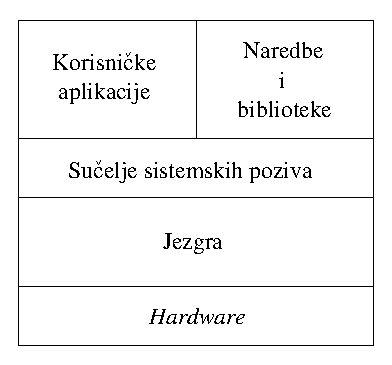
\includegraphics[]{ls_unix}
\end{center}
\caption{Logi�ki slojevi UNIX sustava.}
\label{sl:ls_unix}
\end{figure}

Korisni�ke aplikacije, UNIX naredbe i biblioteke zajedno se nalaze na 
korisni�kom, neprivilegiranom nivou. Programi korisni�kog nivoa se dakle 
izvr�avaju u ograni�enom okru�enju, kontroliranom od strane kernela, koji 
sprje�ava interferenciju programa koji se izvr�avaju istovremeno.


\subsection{Procesi i programi}
\label{subsec:pip}

Program je
def\mbox{}iniran
kao skup naredbi i podataka potrebnih za izvr�avanje neke zada�e. Proces je 
kombinacija programa i trenutnog stanja njegovog izvr�avanja, �to minimalno 
uklju�uje vrijednosti svih varijabli, stanje hardvera i sadr�aj adresnog 
prostora programa. Pojednostavljeno, proces je program u izvr�avanju. Svaki 
UNIX proces ima jedinstveni
identif\mbox{}ikator
zvan
\textit{proces ID},
ili kra�e,
\textit{PID}.
PID je uvijek pozitivna cjelobrojna vrijednost.


\subsection{Mapiranje adresnog prostor procesa i\\ dijeljena memorija}
\label{subsec:mem}

Jezgra je odgovorna za mapiranje adresnog 
(\textit{prividnog} ili
\textit{virtualnog})
prostora procesa na
f\mbox{}izi�ki
adresni prostor ra�unala �to procesu daje privid da mu je na kori�tenje dana 
cjelokupna memorija ra�unala. Kod ve�ine ra�unala mogu�e je da bilo koja 
prividna memorijska
\textit{stranica}
bude
\textit{mapirana}
na bilo koju
f\mbox{}izi�ku
stranicu u memoriji. Na primjer, prividni adresni prostor procesa mo�e biti
mapiran kako je prikazano na 
slici~\ref{sl:mapiranje}.

\begin{figure}
\begin{center}
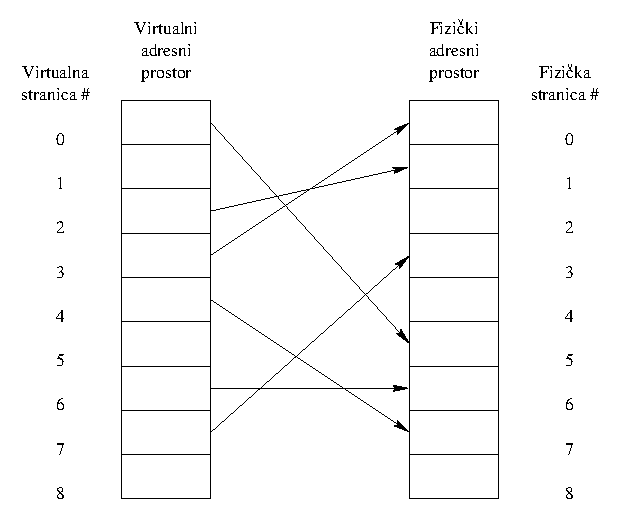
\includegraphics[width = \textwidth]{mapiranje}
\end{center}
\caption{Primjer mapiranja adresnog prostora}
\label{sl:mapiranje}
\end{figure}

Nije nu�no da sve prividne memorijske stranice budu mapirane. Nemapirane
stranice mogu predstavljati neiskori�tene segmente u adresnom prostoru procesa 
ili to mogu biti stranice koje trenutno nisu prisutne u memoriji, ve� se 
nalaze
npr.~na 
\textit{hard disk}-u
ra�unala.

Tako�er, proces ne mora koristiti sve
f\mbox{}izi�ke
stranice prisutne u memoriji. Ove stranice mogu biti dodijeljene drugim 
procesima u sustavu ili uop�e ne  moraju biti kori�tene. U svakom slu�aju, 
proces koji se trenutno izvr�ava ne  smije biti u mogu�nosti da im pristupi.

Odre�ene
f\mbox{}izi�ke
stranice mogu biti dijeljene izme�u nekoliko procesa. U ovom slu�aju kernel 
mapira prividnu stranicu vi�e procesa na istu
f\mbox{}izi�ku 
stranicu. Ove stranice se naj�e��e nazivaju
\textit{segmentima dijeljene memorije}.
Dijeljena memorija slu�i kao mehanizam brze 
komunikacije me�u procesima\footnote{\textit{interprocess communication (IPC)}}
s obzirom da proces mo�e slati podatke bez potrebe izvr�avanja sistemskih
poziva
tj.~upletanja
kernela u prijenos. Kada jedan proces upi�e podatak u dijeljenu memoriju, taj
je istog trena dostupan svim ostalim procesima koji dijele taj memorijski 
segment, odnosno istu
f\mbox{}izi�ku
stranicu.

\subsection{Izmjena konteksta}
\label{subsec:izm_kon}

Kod ve�ine modernih operacijskih sustava, pa tako i kod UNIX-a, procesi se
izvr�avaju
\textit{kvaziparalelno} -
vrijeme izvr�avanja procesa podijeljeno je na kratke vremenske 
odsje�ke, �ija se obrada pravedno izmjenjuje s obradom vremenskih odsje�aka 
drugih trenutno pokrenutih procesa, �to korisnicima sustava daje privid da se
samo njihov proces izvr�ava na ra�unalu. Ovaj �in, u kojem jezgra sustava
trenutno prekida s izvr�avanjem jednog procesa i zapo�inje s izvr�avanjem 
drugog, naziva se
\textit{izmjena konteksta}.
Ovaj pojam uklju�uje pohranu stanja trenutnog procesa kako bi se ovaj
kasnije nastavio, odabiranje novog procesa za izvr�avanje i u�itavanje
pohranjenog procesa u hardver.


\subsection{Signali}
\label{subsec:signali}

Ako proces �elimo obavijestiti o nekom doga�aju, tada mu mo�emo poslati
\textit{signal}.
Na primjer, ako proces dijeli s nulom, jezgra �alje procesu signal �ije je ime 
\texttt{SIGFPE}.
Nakon �to je primio signal, proces mo�e postupiti na jedan od tri na�ina: mo�e
dopustiti da se odigra predvi�ena akcija, mo�e ignorirati signal ili pak
tvorac programa mo�e osigurati vlastitu rutinu koja bi se pozivala prilikom
pojavljivanja odre�enog signala.


\section{Internet komunikacija}
\label{sec:internet}

Uobi�ajeni na�in opisivanja arhitekture mre�e je
ISO-OSI\footnote{\textit{International Organization for Standardization - Open Systems
Interconnection}}
model za ra�unalne komunikacije. Ovo je model sa sedam slojeva, a prikazan je
na 
slici~\ref{sl:isoosi}
zajedno s pribli�no preslikanim
\textit{Internet Protocol Suite}-om\footnote{zajedni�ko ime za TCP/IP 
protokol}.

\begin{figure}
\begin{center}
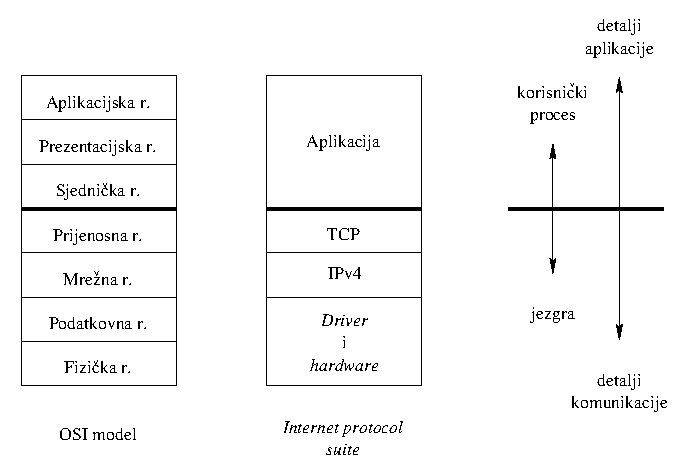
\includegraphics[width = \textwidth]{isoosi}
\end{center}
\caption{Slojevi u OSI modelu i \textit{Internet protocol suite}}
\label{sl:isoosi}
\end{figure}


\subsection{TCP: \textit{Transmission Control Protocol}}

TCP je protokol prijenosne razine Interneta - ostvaruje vezu izme�u krajnjih
korisnika. Rije� je o spojevnom protokolu koji sadr�i mehanizam kontrole
pogre�ki.

Kada TCP �alje podatke na odredi�te, zahtijeva potvrdu njihovog 
primitka. S obzirom da sadr�i algoritme za dinami�ku procjenu
\textit{ukupnog vremena obilaska}\footnote{\textit{round-trip time (RTT)}}
izme�u klijenta i servera zna koliko treba �ekati na potvrdu primitka. Ako 
potvrda ne pristigne, TCP automatski nanovo �alje podatke i �eka du�i 
vremenski rok. 

TCP tako�er vr�i numeraciju paketa koje �alje na odredi�te. Ako paketi ne 
pristignu na cilj redoslijedom kojim su poslani, primatelj ih presla�e prije 
proslje�ivanja aplikaciji. Ako odredi�te slu�ajno primi duple podatke, prema 
brojevima paketa pronalazi koji su podaci duplicirani, te duplicirane segmente
odbacuje.
TCP osigurava i
\textit{prozorsku kontrolu toka}.
Uvijek obznanjuje svome sugovorniku koliko je bajtova spreman primiti.
U bilo kojem trenutku prozor je veli�ina prostora trenutno slobodna u
prijemnom spremniku. Prozor se mijenja s vremenom: kako pristi�u podaci od
po�iljatelja, veli�ina prozora se smanjuje, a kako primaju�a aplikacija �ita
iz spremnika, prozor se pove�ava.

Kona�no, TCP veza je 
\textit{dvosmjerna}
�to zna�i da aplikacija mo�e slati i primati podatke u oba smjera bilo kada
tijekom trajanja veze.


\subsection{IP: \textit{Internet Protocol}}

IP je protokol na mre�noj razini Interneta koji rje�ava adresiranje i
dostupnost svakog ra�unala prisutnog na mre�i. Svako ra�unalo jednozna�no je
odre�eno adresom koja je kod IPv4 protokola velika �etiri bajta, dok pojedinu
uslugu na ra�unalu (npr.~telnet ili ftp) odre�uje
\textit{port}
ili pozitivna broj�ana vrijednost kodirana u dva bajta. Rije� je o bespojnom
protokolu, �to zna�i da ne sadr�i mehanizme oporavka od pogre�ke.

% poglavlje Dizajn

\chapter{Dizajn}

\section{Uvod}

Pod pojmom 
\textit{dizajna softvera} 
podrazumijeva se postupak iznala�enja na�ina pretvaranja
specif\mbox{}ikacije 
programa u funkcionalni program. Bez obzira na odabranu metodologiju,
strukturnu ili objektno orijentiranu, za ovaj proces karakteristi�no je da se
odvija na sljede�im razinama:

\begin{enumerate}
\item
razina:~razlaganje programa na podsustave i
def\mbox{}iniranje
su�elja me�u
njima\footnote{S obzirom da je
cilj ovog rada razvijanje biblioteke klasa namijenjenih realizaciji
komunikacije izme�u procesa, odnosno razvijanje samog podsustava nekog
opse�nijeg budu�eg programa, razumljivo je da je ova razina razlaganja 
prilikom dizajna izostala.}
\item
razina:~razlaganje podsustava na module i opisivanje veza modula s ostatkom
svijeta
\item
razina:~razlaganje modula na rutine i
def\mbox{}iniranje
to�ne sintakse poziva rutina
\item
razina:~unutra�nje dizajniranje rutina
\end{enumerate}

Globalna slika koju dobivamo rje�avaju�i pitanja na vi�im razinama,
poma�e nam da detalje na ni�im razinama sagledamo u pravom kontekstu.
Detalji koje dobivamo rje�avaju�i pitanja na ni�im razinama, osiguravaju
�vrstu podlogu za odluke na vi�i razinama. Skakanje izme�u vi�ih i ni�ih
razina rezultira �vrstom strukturom koja je stabilnija od onih izgra�enih u
cijelosti odozdo prema gore ili obratno. Stoga, dizajniranje je iterativan
postupak temeljen na poku�ajima i pogre�kama.


\section{Objektno orijentirano dizajniranje}
\label{sec:ood}

Osnovna karakteristika objektno orijentiranog dizajniranja je
identif\mbox{}ikacija
stvarnih i apstraktnih objekata koji se onda predstavljaju pomo�u objekata
programskog jezika. Proces se sastoji od
identif\mbox{}ikacije
objekata i klasa objekata,
identif\mbox{}ikacije
operacija nad objektima i klasama, i naposljetku izgradnje sustava iz tih
objekata, klasa i operacija.


\subsection{Klju�ne ideje}

Objektno orijentirano dizajniranje zasniva se na pretpostavci da �e program
biti to bolji �to je modeliran sli�nije realnom problemu kojeg predstavlja.
Koristi nekoliko ideja koje su bitne u suvremenom programiranju.


\subsubsection{Objekti i klase}

Bitna stvar u objektno orijentiranom dizajniranju je razlikovanje objekata i
klasa. Objekt je dinami�ka tvorevina sa
specif\mbox{}i�nim
vrijednostima i
atributima koji su vidljivi kada se program pokrene, dok je klasa stati�na
tvorevina koju vidimo kada pogledamo izvorni
k\^od.
Odnosno, objekt je
specif\mbox{}i�ni
predstavnik neke klase.


\subsubsection{Apstrakcija}

Osnovna prednost apstrakcije je da omogu�ava ignoriranje neva�nih detalja i
koncentriranje na bitne karakteristike.

U strukturnom dizajniranju jedinica apstrakcije je
\textit{funkcija}.
U objektno orijentiranom dizajniranju, to je
\textit{objekt}.
Budu�i da objekt uklju�uje i podatke i pripadaju�e funkcije, omogu�ava
rukovanje ve�im segmentima problema nego �to su same funkcije. Ova �injenica
pove�ava razinu apstrakcije na kojoj se mo�e razmi�ljati, �to zna�i da je
mogu�e intelektualno savladati ve�e dijelove problema bez iziskivanja
dodatnog napora.


\subsubsection{U�ahurivanje}

Pod pojmom u�ahurivanja jedni smatraju �vrsto vezanje podataka i operacija nad
njima u jednu cjelinu (u svrhu kreiranja novog tipa podatka), dok drugima taj
pojam predstavlja skrivanje podataka od dijela
k\^oda
kojemu ti podaci nisu potrebni, odnosno skrivanje detalja implementacije.


\subsubsection{Modularnost}

Grupe srodnih zadataka i podataka grupiraju se u module koji bi trebali, u
idealnom slu�aju, biti dobro povezani iznutra, a imati labave vanjske veze.
Poput skrivanja informacija, cilj je
def\mbox{}inirati
takvo su�elje modula koje se ne�e mijenjati iako se mijenja unutra�njost
modula.


\subsubsection{Hijerarhija i naslje�ivanje}

Pri dizajniranju softverskog sustava, �esto se nailazi na klase koje su
jedne drugima vrlo sli�ne, izuzev nekoliko razlika.
Def\mbox{}iniranje
sli�nosti i razlika me�u takvim klasama naziva se
\textit{naslje�ivanje}.

U objektnom programiranju, naslje�ivanje pojednostavljuje programiranje jer
je mogu�e napisati op�u rutinu za obavljanje bilo �ega �to ovisi samo o
op�im svojstvima neke klase objekata, a onda napisati specijalne rutine koje
�e obavljati specijalne operacije na objektima specijalnih klasa
\textit{deriviranih}
iz op�e (ili
\textit{bazne}).


\subsection{Koraci objektno orijentiranog dizajna}
\label{subsec:koraci_ood}

Koraci navedeni dalje u tekstu ne moraju se nu�no izvoditi redoslijedom u
kojem su izneseni, a �esto se i ponavljaju. Iteracija je va�na kod objektno
orijentiranog dizajniranja kao i kod bilo kojeg drugog dizajnerskog pristupa.

\begin{itemize}
\item \textbf{Identif\mbox{}ikacija objekata i njihovih atributa.}\\
Programi za ra�unala se obi�no zasnivaju na objektima iz realnog svijeta.
Krenuv�i od njih, apstrakcijom dolazimo do softverskih objekata i njihovih
atributa.
\item \textbf{Odre�ivanje �to se mo�e napraviti svakom objektu.}\\
U ovom koraku dolazimo do metoda, odnosno operacija kojih obavljamo nad
objektima pojedine klase.
\item \textbf{Odre�ivanje �to sve objekt mo�e u�initi drugim objektima.}
\item \textbf{Odre�ivanje dijelova svake klase koji �e biti vidljivi.}\\
Jedna od klju�nih dizajnerskih odluka je
identif\mbox{}iciranje
dijelova klasa koji trebaju biti
\textit{javni}
i onih koji trebaju ostati
\textit{privatni}.
Ovu odluku treba donijeti i za podatke i za zadatke.
\item \textbf{Def\mbox{}iniranje su�elja svake klase}\\
Posljednji korak dizajniranja klasa je formalno, sintakti�ko
def\mbox{}iniranje
su�elja svake klase, na razini programskog jezika. Ovo uklju�uje zadatke
koje objekt mo�e izvr�iti kao i naslje�ivanje odnosa izme�u klasa objekata.
Tipi�no, ovo bi uklju�ivalo deklaracije funkcija ili procedura.
\end{itemize}

Nakon prolaska kroz sve korake i stvaranje globalne organizacije objektno
orijentiranog sustava, postupak se ponavlja s dvostrukim ciljem. Ponavlja se
organizacija sustava da bi se dobila bolja organizacija objekata i klasa, a
tako�er se nanovo prolazi kroz sve
def\mbox{}inirane
klase i postupno se razra�uju detalji rje�enja.


\section{Konkretan problem}

Dizajniranje konkretnog zadatka je teklo prema koracima navedenim u prethodnom
odjeljku, no takav redoslijed i nije posve pogodan �to se ti�e �to
jednostavnijeg izno�enja rezultata postupka.
�itav proces, zbog svog iterativnog karaktera, ne�e biti prikazan u cijelosti, 
ve� �e biti izneseno samo njegovo ``kona�no'' rje�enje. Naravno (zahvaljuju�i 
opet iterativnosti) pojam kona�nog dizajna u softverskoj industriji ozna�ava
ne dosezanje krajnje savr�enog, ve� sasvim funkcionalnog rje�enja (i to u
pravilu onog posljednjeg implementiranog prije isteka vremenskog roka
predvi�enog za isporuku proizvoda).


\subsection{Osnovne smjernice}
\label{subsec:osnovne}

Dakle, cilj projekta je realizacija biblioteke klasa u programskom jeziku C++
namijenjene emulaciji paralelnog ra�unala na mre�i radnih stanica.
Ovdje je rije� je o centraliziranom sustavu, �to zna�i da postoji jedan proces 
koji ima
\textit{ovlasti}
ve�e od ostalih, te upravlja njihovim radom, stvara ih i uni�tava. Zbog toga,
taj jedan
\textit{master}
proces ima vezu sa svim ostalim,
\textit{slave}
procesima, dok ti ostali procesi mogu, ali i ne moraju biti povezani s
ostalim, tako�er
\textit{slave}
procesima. Ova situacija je prikazana na
slici~\ref{sl:ms}.

\begin{figure}
\begin{center}
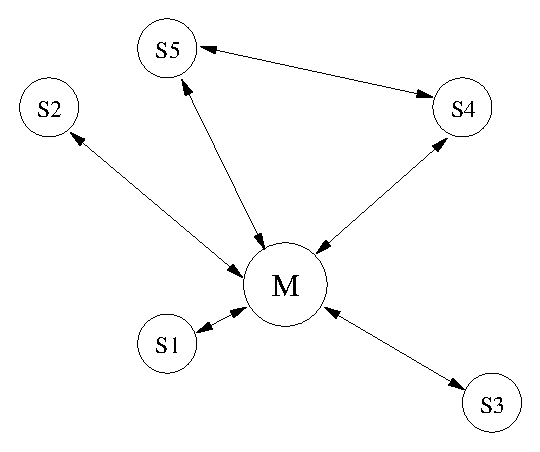
\includegraphics[]{ms}
\end{center}
\caption{Prikaz centraliziranog sustava komunikacije}
\label{sl:ms}
\end{figure}

�to se ti�e same komunikacije, ona mo�e biti realizirana na dva na�ina:
kori�tenjem TCP/IP protokola
(odjeljak~\ref{sec:internet}
na
strani~\pageref{sec:internet})
za procese pokrenute na razli�itim ra�unalima spojenim na Internet, ili putem 
dijeljene memorije
(odjeljak~\ref{subsec:mem}
na
strani~\pageref{subsec:mem})
za procese pokrenute na istom ra�unalu. 

Dizajn komunikacije TCP/IP protokolom ne zahtijeva nikakva dodatna 
obja�njenja jer su njeni detalji na UNIX operacijskim sustavima skriveni nizom
\textit{sistemskih poziva}.
\label{subsec:osn}
Nasuprot tome, komunikacija preko dijeljene memorije iziskuje da joj se
posveti ne�to vi�e pa�nje. Njena realizacija je prikazana na
slici~\ref{sl:sha_mem}.

\begin{figure}
\begin{center}
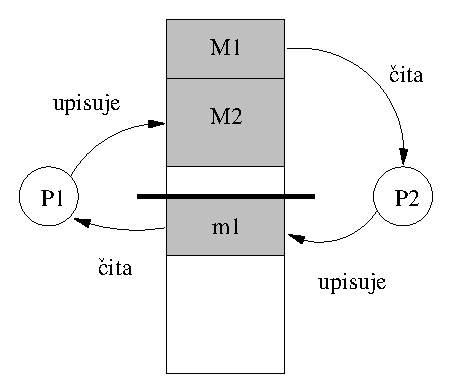
\includegraphics[]{sha_mem}
\end{center}
\caption{Komunikacija putem dijeljene memorije}
\label{sl:sha_mem}
\end{figure}

Zbog jednostavnosti, cjelokupni segment dijeljene memorije je podijeljen u 
dva dijela jednake veli�ine. Dok jedan proces upisuje poruke u jedan dio,
�ita ih iz drugog dijela memorije. Ovo isto vrijedi i za drugi proces samo �to 
ovaj upisuje poruke u dio iz kojeg prvi �ita, a �ita ih iz dijela u kojeg ih 
prvi proces upisuje. 

Nadalje, poruka ne mora biti veli�ine �itavog segmenta u koji se upisuje, 
odnosno iz kojeg se �ita. Zbog toga, svaki proces koji komunicira dijeljenom
memorijom ima po dva
\textit{pokaziva�a} -
jedan za pisanje, a drugi za �itanje. Nakon �to proces npr.~upi�e poruku,
pokaziva� za pisanje se pomi�e na prvo sljede�e slobodno mjesto u memoriji 
koje je spremno primiti poruku. U slu�aju da je �itav segment memorije
predvi�en za upisivanje popunjen, pokaziva� se vra�a na po�etak segmenta
gdje �eka da drugi proces oslobodi memoriju nakon �to pro�ita poruku. Na
ovaj na�in je realiziran
\textit{cirkularni spremnik}.
Posve analogna situacija vrijedi i za �itanje poruka - nakon �to je poruka
pro�itana, pokaziva� se pomi�e na mjesto na kojem proces o�ekuje prvu sljede�u
poruku. Kada ovaj pokaziva� stigne do kraja svog segmenta, tako�er se vra�a
na njegov po�etak.


\subsection{Identif\mbox{}ikacija klasa i opisivanje njihovih me�usobnih veza}

S obzirom na izneseno u prethodnom odjeljku, i na prvi pogled jasno iska�u
sljede�i pojmovi iz
\textit{realnog svijeta}:
\textit{proces, veza}
i
\textit{poruka}.
Ovi pojmovi preslikani su u klase
\texttt{Process},
\texttt{Connection}
i
\texttt{Message}\footnote{U programerskoj praksi tipi�no je imenovanje
varijabli, funkcija pa tako i korisni�kih tipova podataka na engleskom
jeziku.}.\\

Razmotrimo li klasu
\texttt{Process}
podrobnije, uo�avamo da je njen pojam preop�enit �to bi uzrokovalo njenu
glomaznost i, u fazi implementacije, probleme. Stoga je klasa
\texttt{Process}
idealan kandidat za baznu klasu iz koje bi bili derivirani
specif\mbox{}i�ni
vidovi pojma
\textit{proces}
sa svojim
specif\mbox{}i�nim
detaljima. O�ito je da �e te
specif\mbox{}i�ne
klase biti
\texttt{MasterProcess}
i
\texttt{SlaveProcess}.

Jedna od zada�a objekta klase
\texttt{MasterProcess}
je kreiranje objekata klase
\texttt{SlaveProcess}.
S obzirom da se ovaj postupak ne mo�e implementirati na na�in da se odvije u 
jednom koraku, ovi detalji kreiranja su skriveni u klasi
\texttt{Child} koja na neki na�in predstavlja
``prijelazno stanje''
klase
\texttt{SlaveProcess}.

Tako�er, klasa
\texttt{Process}
se mo�e dalje rasteretiti odvajanjem onog dijela funkcionalnosti koji je
odgovoran za obradu pristiglih poruka. Ovu funkcionalnost sadr�i klasa
\texttt{MessageProcessor}.\\

Klasa
\texttt{Connection}
je tako�er preop�enita s obzirom da mogu postojati dvije vrste veza izme�u
procesa - stoga su uvedene klase
\texttt{SharedMem}
i
\texttt{TCPConnection}
koje konkretiziraju pojam
\textit{veze}.

Dalje, promatraju�i klasu
\texttt{SharedMem}
dolazimo i do klase
\texttt{CircularPtr},
odnosno
\textit{cirkularnog pokaziva�a}
�ije je uvo�enje opravdano opisom u prethodnom odjeljku.

Tijekom implementacije, pojavila se i potreba za uvo�enjem jo� jedne klase
derivirane iz klase
\texttt{Connection}
u svrhu ozna�avanja veze koja je tijekom izvo�enja programa uni�tena.
U ovom slu�aju, rije� je o klasi
\texttt{Destroyed}.\\

Naposljetku, za potrebe sno�enja s pojavom iznimnih situacija (npr.~slanja
poruka zatvorenom vezom) tijekom rada programa, stvorena je jo� jedna klasa
imena
\texttt{Exception}.\\

Glavna zada�a baznih klasa
\texttt{Process}
i
\texttt{Connection}
je
def\mbox{}iniranje
su�elja koje klase derivirane iz njih implementiraju, svaka na svoj na�in.
Tako ako npr.~od objekta klase
\texttt{Process}
zatra�imo odre�enu akciju, ova �e biti izvr�ena ili na na�in kako je
implementira klasa
\texttt{MasterProcess}
ili na na�in kako je implementira klasa
\texttt{SlaveProcess},
ovisno o tome kojoj objekt pripada.\newpage

Upravo
def\mbox{}iniran
globalan dizajn prikazan je na
slici~\ref{sl:c_dia}
UML\footnote{\textit{Unif\mbox{}ied Modeling Language} - jezik namijenjen
modeliranju kod objektno orijentiranih programskih jezika}
dijagramom. Klasa
\texttt{exception}
je dio standardne biblioteke programskog jezika C++.

\begin{figure}
\begin{center}
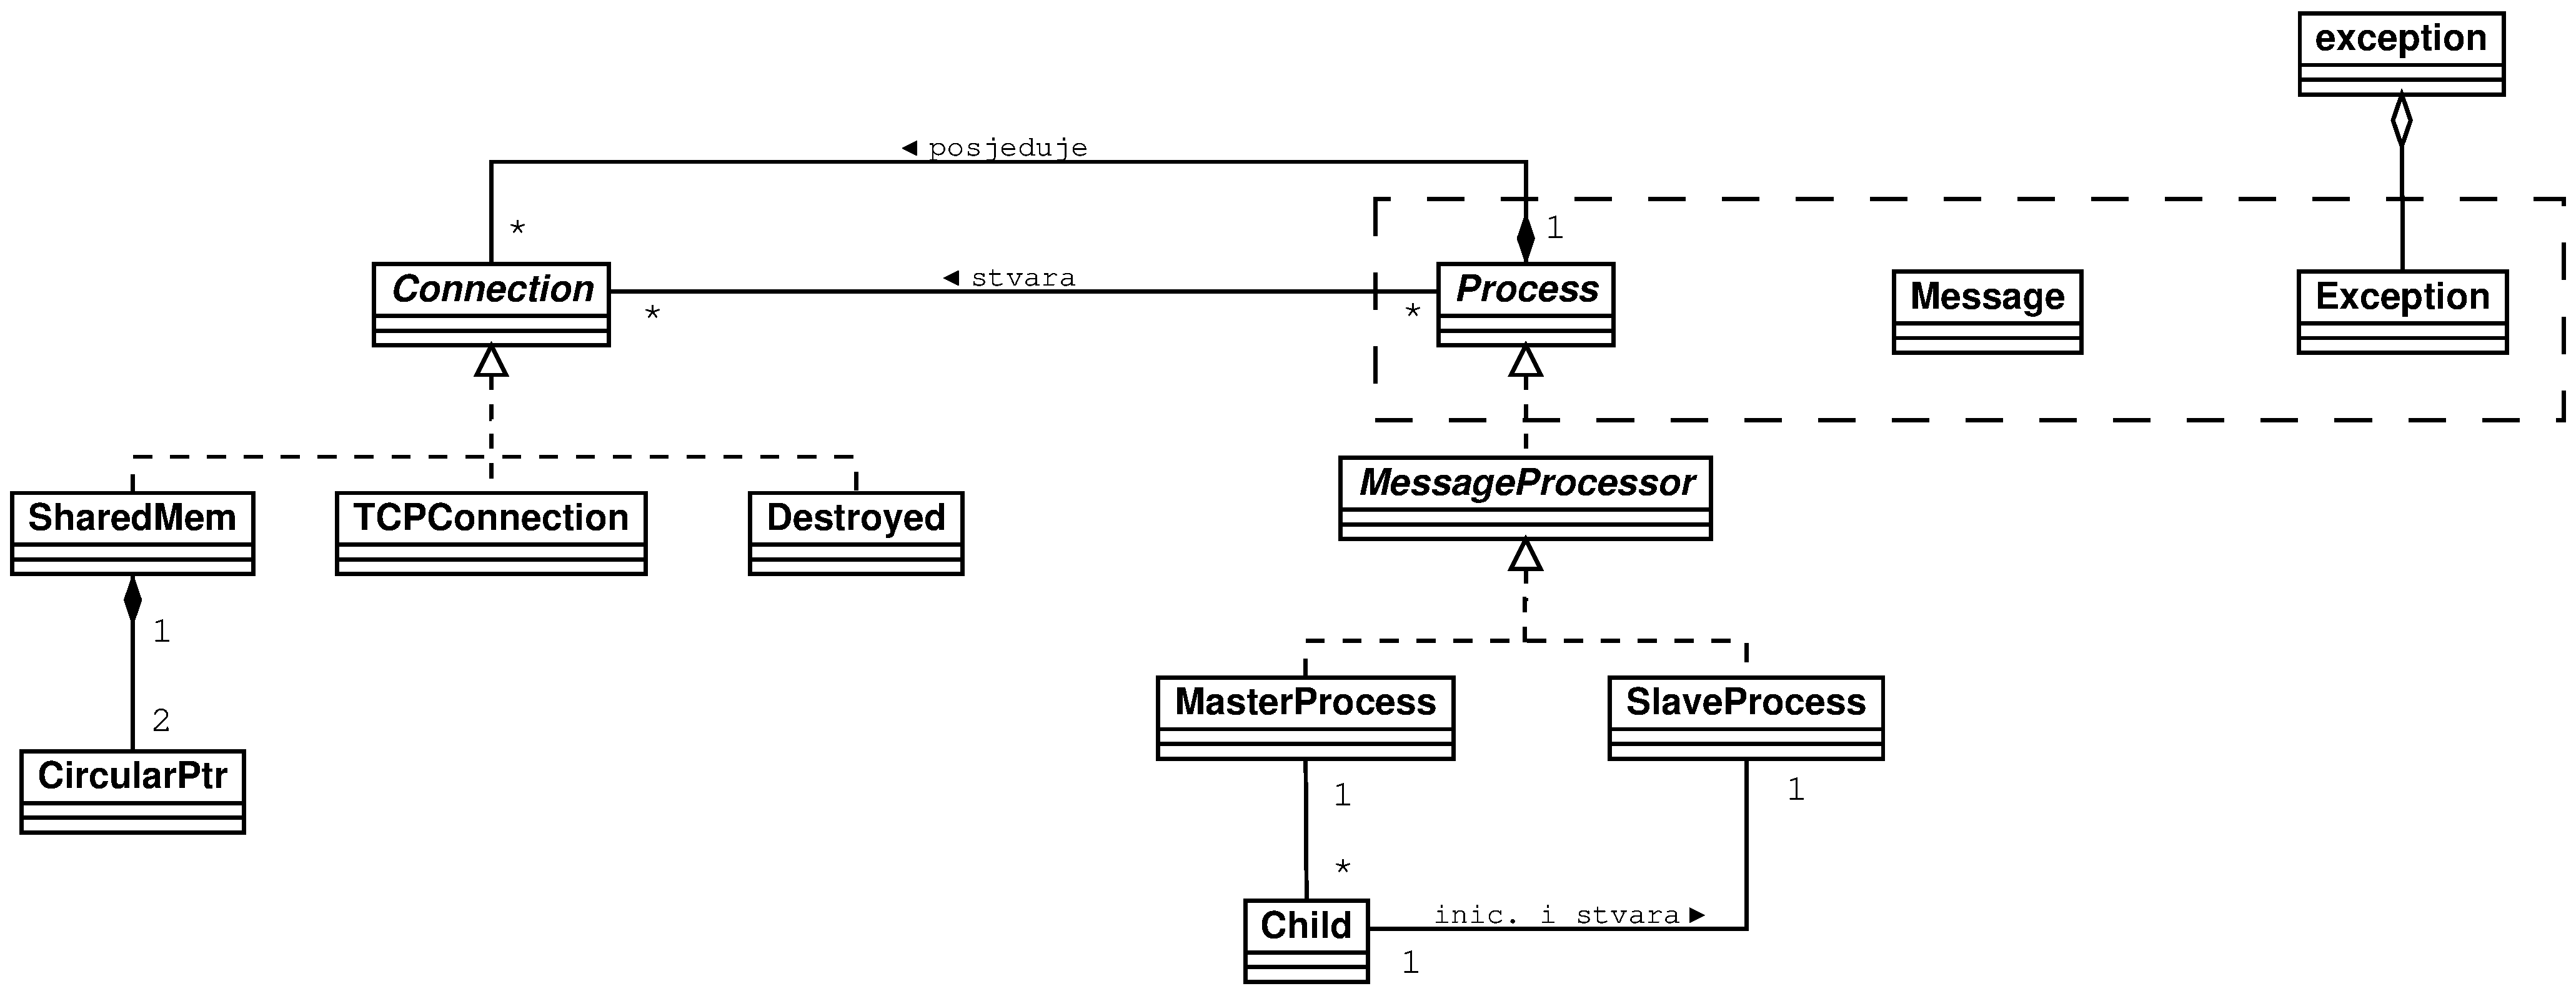
\includegraphics[angle = 90, height = \textheight]{c_dia}
\end{center}
\caption{\textit{UML class} dijagram}
\label{sl:c_dia}
\end{figure}


\subsection{Opis \textit{API}-ja}

S obzirom na postoje�ih jedanaest klasa, opis ostalih koraka
objektno orijentiranog dizajna za svaku od njih zauzeo bi previ�e prostora.
Zbog toga slijedi opis
\textit{API}-ja,
odnosno
def\mbox{}iniranje
su�elja onih klasa koje su vidljive korisniku biblioteke. Na
slici~\ref{sl:c_dia}
te su klase obuhva�ene iscrtkanim pravokutnikom.

\subsubsection{Klasa \texttt{Process}}

Metode klase
\texttt{Process}
su sljede�e:

\begin{itemize}
\item
\textit{konstruktor}
(zadu�en za kreiranje objekta) i
\textit{destruktor}
(zadu�en za uni�tavanje objekta) ne zahtijevaju
daljnja poja�njenja. Va�no je samo napomenuti da konstruktor kao parametar
prima pokaziva� na znakovni niz koji sadr�i ime izvr�ne datoteke, no
korisnik se ne mora time optere�ivati s obzirom da je za kreiranje objekta 
zadu�ena posebna funkcija
\texttt{start\_new}
o kojoj �e naknadno biti jo� rije�i.
\item
Metoda
\texttt{name}
vra�a pokaziva� na znakovni niz koji sadr�i ime izvr�ne datoteke, a ne prima
nikakve parametre.
\item
\texttt{send},
kao �to samo ime ka�e, �alje poruku drugom procesu. Funkcija prima dva
parametra od kojih je prvi redni broj veze kojom se �alje poruka, dok je
drugi
\textit{referenca}
na poruku (objekt klase
\texttt{Message})
koja se �alje. Ova metoda vra�a jednu od dvije mogu�e vrijednost
ovisno da li je poruka uspje�no poslana ili je poku�ana poslati vezom koja
je u me�uvremenu uni�tena (proces na drugoj strani veze vi�e ne postoji).
\item
Metoda
\texttt{receive}
tako�er prima dva parametra. Prvi je broj veze s koje proces �ita poruku,
dok je drugi pokaziva� na objekt klase
\texttt{Message}
u koji �e pristigla poruka biti upisana.
\texttt{receive}
tako�er i vra�a jednu od dvije vrijednosti, ovisno da li je pristigla kakva
poruka tom vezom prilikom poziva te funkcije ili ne.
\item
Tu su i dvije metode
\texttt{start\_new}
od kojih prva ne prima nikakav parametar i slu�i za pokretanje procesa na
istom ra�unalu, dok druga kao parametar prima pokaziva� na znakovni niz koji
sadr�i ime ra�unala na mre�i na kojem �e se pokrenuti novi proces, te
\textit{direktorij}
s imenom izvr�ne datoteke novog procesa.
\item
Metoda
\texttt{kill},
kao �to to i samo ime govori, slu�i za
\textit{ubijanje}
procesa, pa kao svoj parametar prima redni broj veze s doti�nim procesom.
\item
\texttt{route}
je zadu�ena za stvaranje veze izme�u dvaju
\textit{slave}
procesa. Kao svoja dva parametra prima redne brojeve veza procesa izme�u
kojih se ostvaruje nova veza. Ova funkcija vra�a logi�ku vrijednost ovisno o
tome da li je nova veza ostvarena ili ne. Ta vra�ena vrijednost ima smisla
samo kod
\texttt{MasterProcess}-a
jer dok on direktno stvara novu vezu, zbog centraliziranosti, instance klase
\texttt{SlaveProcess}
samo podnose zahtjev
\texttt{MasterProcess}-u
koji ga realizira.
\item
\texttt{master}
i
\texttt{slave}
metode vra�aju logi�ku vrijednost ovisno da li objekt pripada klasi
\texttt{MasterProcess},
odnosno klasi
\texttt{SlaveProcess}.
\item
Metoda
\texttt{loop}
prolazi jednom kroz sve veze jednog procesa provjeravaju�i da li je stigla 
kakva poruka bilo kojom od njih. U slu�aju da jest, ova metoda automatski 
obra�uje pristiglu poruku. U slu�aju da nema nove poruke, funkcija ne �eka
da se ova pojavi ve� odmah provjerava sljede�u vezu.
\texttt{loop}
vra�a logi�ku vrijednost koja indicira da li bi u sljede�em prolazu moglo biti
jo� pristiglih poruka ili ne.
\item
Kona�no, metoda
\texttt{loop\_forever}
uvodi proces u
\texttt{pasivno}
stanje u kojem je njegova jedina zada�a da prima i obra�uje pristigle poruke
sve dok ne primi zahtjev za prestankom rada.
\end{itemize}

\textit{API}
klase
\texttt{Process}
nalazi se na
slici~\ref{sl:process}.

\begin{figure}
\begin{center}
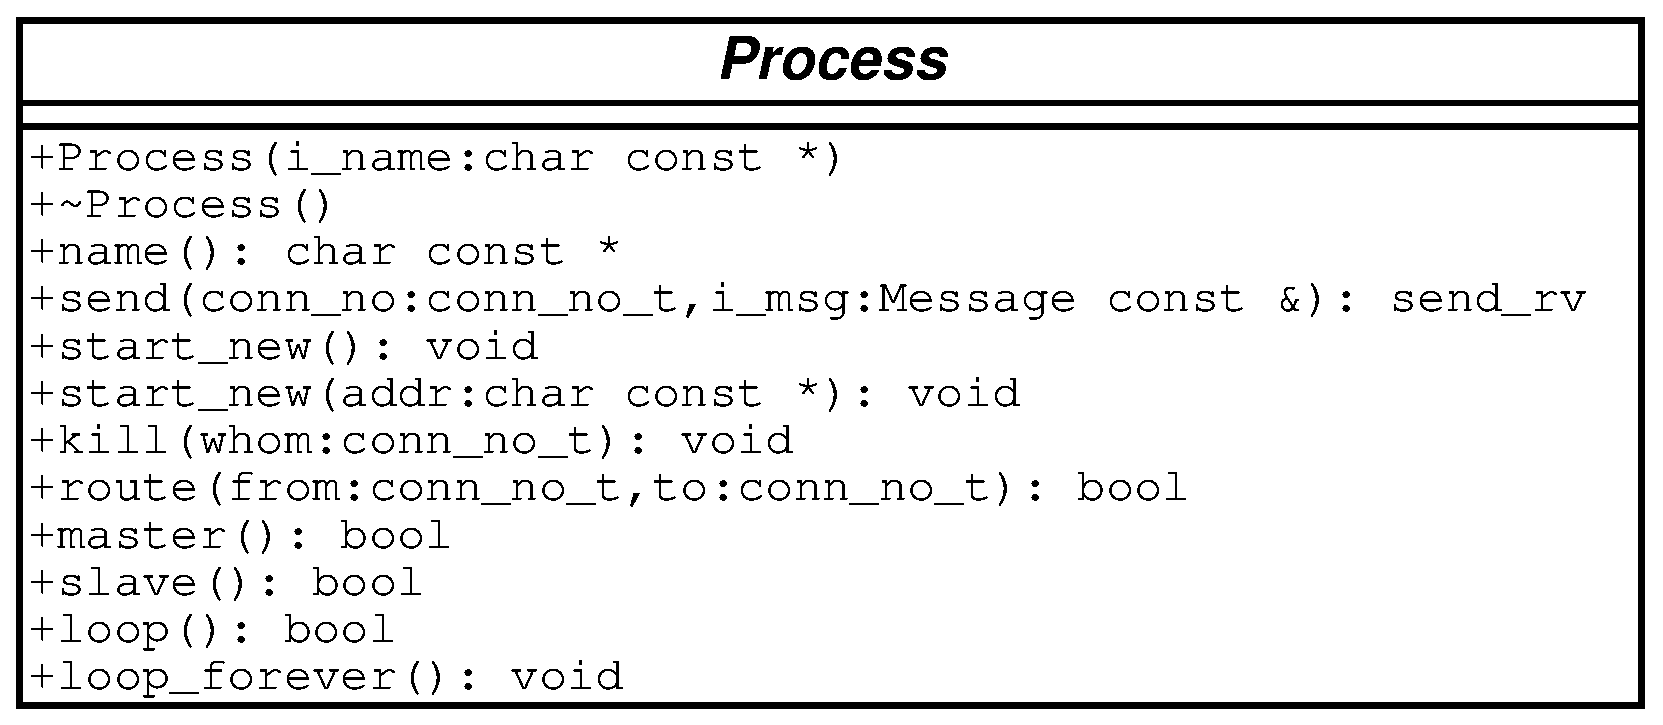
\includegraphics[width = 0.7\textwidth]{Process}
\end{center}
\caption{\textit{API} klase \texttt{Process}}
\label{sl:process}
\end{figure}


\subsubsection{Klasa \texttt{Message}}

\begin{itemize}
\item
Klasa
\texttt{Message}
posjeduje �etiri konstruktora.
Prvi,
\textit{default}
konstruktor prima od jednog do tri parametra. Prvi je cjelobrojni
identif\mbox{}ikacijski
broj poruke, drugi je pozitivan cijeli broj koji opisuje
du�inu poruke u bajtovima i tre�i je pokaziva� na memorijsku lokaciju na
kojoj se nalaze podaci koji �e formirati samo tijelo poruke.

Drugi, takozvani
\textit{copy}
konstruktor je uveden zbog discipliniranosti u programiranju s obzirom na
karakter klase.

Ostali konstruktori su sli�ni
\textit{copy}
konstruktoru. Prvi od njih kao parametre prima referencu na objekt klase
\texttt{Message} i cjelobrojnu vrijednost koja predstavlja novi ID poruke.
Naime, ovaj konstruktor od ve� postoje�e poruke (prvog parametra) stvara
novu poruku potpuno iste du�ine i sadr�aja s tim da je jedina razlika izme�u
njihovih
identif\mbox{}ikacijskih
brojeva (drugi parametar). Naredni
\textit{copy}
konstruktor tako�er stvara novu poruku od stare, s time da tijelo nove
poruke sadr�i samo jedan segment tijela stare. Dakle, ovaj konstruktor
prima �etiri parametra. Prvi i drugi parametar su posve isti kao
i kod prethodnog konstruktora, tre�i parametar je cjeli broj koji
predstavlja pomak u bajtovima od po�etka tijela originalne poruke, a �etvrti je
broj bajtova koji �e �initi tijelo nove poruke.
\item
Sljede�a metoda je
\textit{overload}-ani
\texttt{operator=}
koji je tu tako�er zbog discipliniranosti u programiranju.
\item
\texttt{copy\_data\_to}
je funkcija zadu�ena za kopiranje tijela poruke na novu memorijsku lokaciju
�iju adresu korisnik proslje�uje kao jedini parametar ove funkcije. Ova
metoda, nakon �to obavi svoj zadatak, tako�er i vra�a taj pokaziva�, �ime je
postignuta sli�nost sa sintaksom funkcija iz standardne biblioteke.
\item
\texttt{compare\_data}
uspore�uje memorijski segment (njegova adresa je prvi parametar funkcije)
s tijelom poruke. Usporedba se vr�i samo za broj bajtova koji je proslije�en
kao drugi parametar. Ova funkcija vra�a vrijednost razli�itu od nule ako se 
uspore�eni segmenti razlikuju, odnosno nulu, ako su segmenti jednakog sadr�aja.
\item
\texttt{int\_data\_at}
vra�a cjelobrojnu vrijednost, 
(\textit{integer})
koja se nalazi u tijelu poruke na onom rednom mjestu koje je jednako jedinom
parametru funkcije.
\item
Metoda
\texttt{char\_data\_at}
jednaka je gorespomenutoj, samo �to vra�a jedan bajt, odnosno
\textit{character}.
\item
\texttt{mid}
metoda ne prima nikakve parametre, a daje
identif\mbox{}ikacijski
broj poruke.
\item
\texttt{len}
tako�er ne prima parametre, a vra�a du�inu tijela poruke u bajtovima.
\end{itemize}

\textit{API}
klase
\texttt{Message}
nalazi se na
slici~\ref{sl:Message}.

\begin{figure}
\begin{center}
\includegraphics[width = \textwidth]{Message}
\end{center}
\caption{\textit{API} klase \texttt{Message}}
\label{sl:Message}
\end{figure}


\subsubsection{Klasa \texttt{Exception}}

Klasa
\texttt{Exception}
derivirana je iz standardne klase
\texttt{exeption}
pa je opis njenog
\textit{API}-ja
ne�to kra�i jer klasa ima svega jednu metodu (izuzmu li se konstruktor i
destruktor).

\begin{itemize}
\item
Konstruktor i destruktor ne iziskuju dodatna obja�njenja. Va�no je samo
naglasiti da konstruktor kao svoj parametar prima pokaziva� na znakovni niz
koji opisuje iznimnu situaciju koja se dogodila.
\item
Metoda
\texttt{what}
ne prima nikakvih parametara, a vra�a pokaziva� na znakovni niz koji daje
opis iznimke.
\end{itemize}

\textit{API}
klase
\texttt{Exception}
prikazan je na
slici~\ref{sl:exception}.

\begin{figure}
\begin{center}
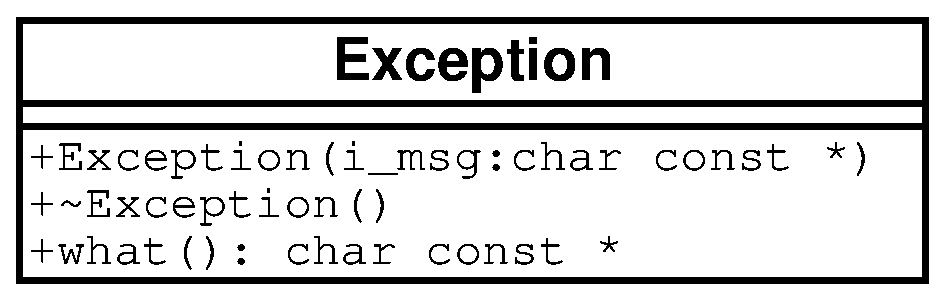
\includegraphics[width = 0.5\textwidth]{Exception}
\end{center}
\caption{\textit{API} klase \texttt{Exception}}
\label{sl:exception}
\end{figure}

\newpage


\section{C++ specif\mbox{}i�nosti}
\subsection{Skrivanje implementacije\\(\textit{Cheshire Cat design pattern})}
\label{subsec:si}

U svrhu potpunog skrivanja implementacije od korisnika biblioteke, te zbog
smanjenja kompilacije tijekom razvojne faze, kori�tene su
\textit{handle classes}
odnosno
\textit{Cheshire Cat design pattern}.
S obzirom da je ova tehnika kori�tena pri dizajnu svih klasa biblioteke,
zaslu�uje kratak opis.
Kontrola pristupa u C++-u nam omogu�ava da odvojimo su�elje od
implementacije, ali skrivanje implementacije nije potpuno - osim metoda u
\textit{header}
datotekama izlo�eni su i atributi klase. Ovaj slu�aj je vidljiv na
slici~\ref{sl:neskriveno}.

\begin{figure}
\begin{center}
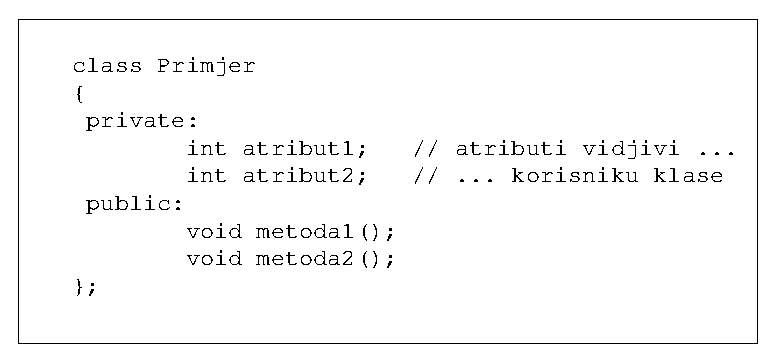
\includegraphics[width = 0.7\textwidth]{neskriveno}
\end{center}
\caption{Primjer deklaracije klase u C++-u}
\label{sl:neskriveno}
\end{figure}

Premda korisnik nije u ovom primjeru u stanju da pristupi varijablama
\texttt{atribut1}
i
\texttt{atribut2},
on ih dalje vidi. Da bi se korisnik u potpunosti rasteretio detalja
implementacije, ovom problemu se dosko�ilo na sljede�i na�in - svi atributi 
klase zamijenjeni su pokaziva�em na nepotpuno
specif\mbox{}iciranu
\textit{strukturu}
(ili klasu) koja je
def\mbox{}inirana
ne vi�e u
\textit{header}-u
ve� u datoteci zajedno s implementacijom. Kao �to je prikazano na
slici~\ref{sl:skriveno},
korisnik je sada svjestan samo metoda klase, pa i njegovo razumijevanje iste
nije ometano prisutno��u njemu nepotrebnih detalja.

\begin{figure}
\begin{center}
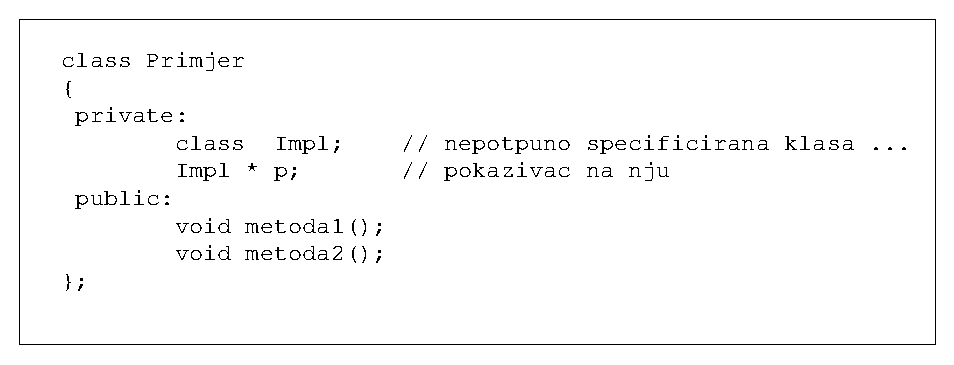
\includegraphics[width = 0.7\textwidth]{skriveno}
\end{center}
\caption{Primjer primjene \textit{Cheshire Cat design pattern}-a}
\label{sl:skriveno}
\end{figure}

\chapter{Implementacija}

\section{Uvod}

S obzirom na veli�inu projekta, izno�enje postupka implementacije �itavog
k\^oda
oduzelo bi previ�e prostora i vremena. Stoga �e u ovom poglavlju isklju�ivo
biti rije�i o problemima koji su tijekom implementiranja iziskivali vi�e
pa�nje, poput postupka inicijalizacije novih procesa, komunikacije putem
dijeljene memorije te komunikacije TCP/IP protokolom.


\section{Inicijalizacija procesa}

Postavlja se pitanje kako prilikom pokretanja proces zna da li mu je
namijenjena uloga
\texttt{MasterProcess}-a
ili nekog od
\texttt{SlaveProcess}-a.
Ovo raspoznavanje je implementirano kori�tenjem
\textit{argumenata komandne linije}
preko kojih svaki proces ispituje da li je pokrenut iz
\textit{konzole}
ili iz nekog drugog procesa. Naime
\texttt{MasterProcess}
kao jedan od argumenata komandne linije ostalim procesima proslje�uje
poseban znakovni niz koji izme�u ostalog sadr�i i njegov
PID\footnote{Pojam PID-a je obja�njen u odjeljku~\ref{subsec:pip}}.
Tek pokrenuti proces uspore�uje taj primljeni PID s PID-om procesa koji ga je
kreirao. Ako su oba broja ista, tada novi proces zna da mu je namijenjena uloga
\texttt{SlaveProcess}-a.
Sav ovaj postupak implementiran je, izme�u ostalog, u inicijalizacijskoj
funkciji
\texttt{start\_new}.
Ova funkcija prima tri parametra od kojih su prva dva parametri koje
operacijski sustav proslje�uje procesu (argumenti komandne linije) dok tre�i
parametar predstavlja pokaziva� na funkciju namijenjenu obradi korisni�kih
poruka. Funkcija
\texttt{start\_new}
vra�a pokaziva� na kreirani objekt klase
\texttt{MasterProcess}
odnosno
\texttt{SlaveProcess}.
Preko ovog pokaziva�a vr�e se svi daljnji pozivi metoda ovog objekta.
Tako�er, kori�tenjem posebnog broja�a onemogu�eno je kreiranje vi�e instanci
ovih klasa po jednom procesu.


\section{Izbjegavanje \textit{aktivnog �ekanja}}

Posve je mogu� scenarij u kojem jedan proces �eka drugog da ovaj obavi svoj
posao. Najjednostavniju implementaciju ovog �ekanja bi predstavljala iteracija
u praznoj petlji. No mana ovog rje�enja je u tome �to i iteriranje kroz praznu
petlju predstavlja nekakvu aktivnost
(tzv.~\textit{aktivno �ekanje}),
te se na taj na�in i dalje tro�i procesorsko vrijeme koje bi drugi procesi
znali bolje iskoristiti. Ovom problemu je dosko�eno na na�in da se proces
koji �eka
\textit{po�alje na spavanje}
pozivom standardne funkcije
\texttt{usleep}
koja kao parametar prima broj mikrosekunda koje �e proces provesti
\textit{spavaju�i}.
Pri implementaciji je kao parametar u svim pozivima ove funkcije kori�tena
jedinica �to je dovoljno da se prouzro�i
izmjena konteksta\footnote{Upoznavanje s ovim pojmom je bilo u
odjeljku~\ref{subsec:izm_kon}}.
Kori�tenje ove rutine mo�e se primijetiti na
slici~\ref{sl:lock}
kod implementacije Dekkerovog algoritma obja�njenog u
odjeljku~\ref{subsec:dekker}.
Tako�er, da bi se postigle bolje performanse, svaki proces nakon slanja poruke
drugom procesu tako�er �alje i
\textit{signal}\footnote{Pojam \textit{signala} je uveden u
odjeljku~\ref{subsec:signali}}
koji
\textit{budi}
primatelja u slu�aju da je ovaj
\textit{na spavanju}.
Kao signal je odabran
\texttt{SIGUSR2}
s obzirom da kod primanja
\texttt{SIGIO}
signala dolaze do izra�aja razlike me�u implementacijama razli�itih verzija
UNIX-a.


\section{Detalji implementacije komunikacije dijeljenom memorijom}

Najosnovnije crte komunikacije dijeljenom memorijom dane su u
odjeljku~\ref{subsec:osn}
na
strani~\pageref{subsec:osn}.
Slijedi ne�to vi�e o samim porukama i ostvarivanju veza izme�u procesa.


\subsection{Razmjena poruka}

Ve� je bilo spomenuto da dijeljeni memorijski segment predstavlja dva
\textit{cirkularna spremnika}. Procesi upisuju poruke svaki u svoj spremnik
sve dok ne do�u do njegovog kraja. Tada se vra�aju opet na njegov po�etak i
ponavljaju �itavu stvar s jednim izuzetkom - prilikom svakog sljede�eg
upisivanja procesi provjeravaju da li je poruka koja je u pro�lom ciklusu
bila upisana na tom mjestu pro�itana. U slu�aju da nije, proces koji
poku�ava upisati novu poruku odga�a svoj naum sve dok se ve� upisana poruka
ne pro�ita. S obzirom na izneseni problem, proces koji upisuje poruke mora
pamtiti memorijske adrese na kojima se one nalaze da bi kasnije mogao
provjeriti da li su doti�ne poruke pro�itane ili ne. Ovaj zadatak
je jednostavno implementiran kori�tenjem
\textit{STL}\footnote{\textit{Standard Template Library}}
\textit{container}-a
zvanog
\textit{deque}.
Deque je struktura koju je najlak�e do�arati �pilom karata. Karte
najjednostavnije mo�emo umetati i izbacivati iz �pila sa njegovog prednjeg ili
stra�njeg kraja. U ovom se slu�aju, kako se poruke upisuju, na kraj deque-a
dodaju njihove memorijske adrese. Nakon �to je pro�ao jedan �itav ciklus,
prilikom svakog sljede�eg upisivanja proces provjerava poruke na adresama
koje se nalaze isklju�ivo na samom po�etku deque-a. Da li je odre�ena poruka
pro�itana ili ne, procesi odre�uju na temelju jedne od varijabli iz
zaglavlja poruke, koja je (zajedno s �itavim zaglavljem) opisana ne�to ni�e u
tekstu.\\

U trenutnoj implementaciji, poruke koje se razmjenjuju dijeljenom memorijom
ograni�ene su svojom veli�inom. Cjelokupni segment dijeljene memorije veli�ine
je jedne memorijske
\textit{stranice}
koja kod ve�ine UNIX implementacija iznosi �etiri kilobajta. Segment je
prema~\ref{subsec:osn}
podijeljen u dva dijela �to zna�i da cjelokupna poruka mo�e maksimalno biti
duga dva kilobajta. Od ova dva kilobajta 24 bajta otpadaju na zaglavlje
poruke �to zna�i da korisnikovi podaci, odnosno tijelo poruke, mogu
maksimalno biti dugi 2024 bajta
(slika~\ref{sl:message}).
Varijable
\texttt{turn},
\texttt{status[0]}
i
\texttt{status[1]}
slu�e za sinhronizaciju pristupa dijeljenoj memoriji. Naime, sasvim je mogu�e
da jedan proces zapo�ne s upisivanjem poruke, ali tada zbog izmjene konteksta
(\ref{subsec:izm_kon})
privremeno bude prekinut s radom te se umjesto njega nastavi izvr�avati neki
drugi proces. Redoslijed izmjene konteksta mo�e biti upravo takav da proces
koji �ita poruke pristupi dijeljenoj memoriji i pro�ita poruku koja nije do
kraja upisana, pa stoga ni valjana. Rje�enje ovog problema i svrha ovih triju
sinhronizacijskih varijabli detaljno su opisani u
odjeljku~\ref{subsec:dekker}.
Dakle, s obzirom da svaka poruka ima vlastite sinhronizacijske varijable,
o�ito je da je sinhronizacija realizirana na
\textit{razini poruka},
�to zna�i da jedan proces mo�e �itati jednu poruku dok u istom memorijskom
segmentu drugi proces upisuje drugu poruku.

Varijabla
\texttt{fresh}
je tako�er svojstvena komunikaciji putem dijeljene memorije. Nakon �to jedan
proces upi�e poruku, vrijednost ove varijable obavezno postavlja u jedinicu
�to zna�i da je poruka
\textit{svje�a},
odnosno da jo� nije pro�itana. Kada drugi proces pro�ita poruku, njeno mjesto
u dijeljenoj memoriji popunjava nulama �ime i vrijednost
\texttt{fresh}
varijable postavlja na nulu. Na ovaj na�in proces koji je upisao poruku mo�e
saznati da je ova pro�itana te da na njeno mjesto mo�e upisati novu, kao �to je
ve� bilo opisano.

Varijable
\texttt{mid}
(odnosno
identif\mbox{}ikacijski
broj poruke) i
\texttt{len}
(du�ina tijela poruke) ne iziskuju daljnja poja�njenja. Va�no je samo
napomenuti da procesi mogu razmjenjivati poruke du�ine tijela od nula bajtova,
dakle sama zaglavlja, pa je stoga na
slici~\ref{sl:message}
tijelo poruke, tj.~segment s podacima, prikazan u zagradama.\newpage

\begin{figure}
\begin{center}

\includegraphics[]{message}
\caption{Poruka upisana u dijeljenu memoriju}
\label{sl:message}
\end{center}
\end{figure}


\subsection{Kreiranje novog procesa}
\label{subsec:knp}

Objekt klase
\texttt{MasterProcess},
prije kreiranja
\texttt{SlaveProcess}-a,
s kojim ima namjeru ostvariti ovaj vid komunikacije, od operacijskog sustava
zatra�i da mu se dodijeli segment dijeljene memorije pozivaju�i funkciju
\texttt{shmget}.
Spomenuta funkcija vra�a
identif\mbox{}ikator
dijeljenog segmenta kojeg nadalje
\texttt{MasterProcess}
koristi kao argument funkcije
\texttt{shmat}
koja vr�i mapiranje dijeljenog memorijskog segmenta na virtualni adresni
prostor procesa
(odjeljak~\ref{subsec:mem}
na
strani~\pageref{subsec:mem}).
Nakon �to je segment mapiran popunjen je nepoznatim vrijednostima koje su se
tog trenutka na�le na tom mjestu u memoriji
(tzv.~\textit{garbage value}).
Zbog toga prije i�eg drugog,
\texttt{MasterProcess}
bri�e sve �to se nalazi u mapiranom segmentu, to�nije, sve vrijednosti u
njemu postavlja na nule. �itav ovaj proces na
slici~\ref{sl:start_new}
predstavlja
\textit{korak 1}.
Tek sada
(\textit{korak 2})
\texttt{MasterProcess}
kreira novi objekt klase
\texttt{SlaveProcess}
kojemu proslje�uje
identif\mbox{}ikacijski
broj segmenta dijeljene memorije kao
jedan od
\textit{argumenata komandne linije}.
Nakon �to je
\texttt{SlaveProcess}
kreiran poziva funkciju
\texttt{shmat}
kojoj kao parametar proslje�uje primljeni
identif\mbox{}ikacijski
broj �ime se
segment dijeljene memorije mapira i na virtualni adresni prostor
\texttt{SlaveProcess}-a.
Naposljetku,
isklju�ivo da bi dojavio
\texttt{MasterProcess}-u
kako je kreiran te kako se uspje�no
\textit{prika�io}
na segment dijeljene memorije,
\texttt{SlaveProcess}
upravo tim segmentom �alje prvu poruku.

\begin{figure}
\begin{center}
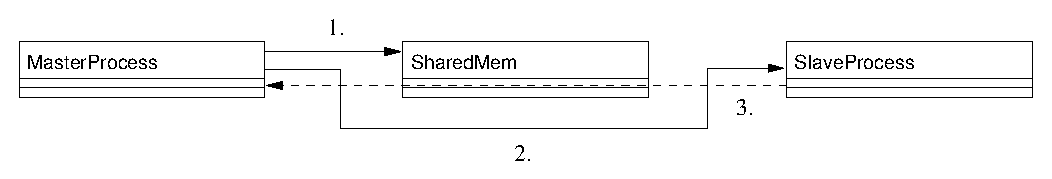
\includegraphics[width = \textwidth]{start_new}
\caption{Kreiranje novog procesa na istom ra�unalu}
\label{sl:start_new}
\end{center}
\end{figure}

Va�no je napomenuti da se funkcija za kreiranje dijeljenog memorijskog segmenta
\texttt{shmget},
te funkcija za mapiranje tog segmenta u virtualni adresni prostor procesa
\texttt{shmat},
pozivaju iz konstruktora klase
\texttt{SharedMem}.
Ovo zna�i da ih ni
\texttt{MasterProcess}
ni
\texttt{SlaveProcess}
ne pozivaju direktno, ve� kreiraju novi
\texttt{SharedMem}
objekt koji dalje sam vodi ra�una o �itavom postupku.


\subsection{Stvaranje veze izme�u dvaju \texttt{SlaveProcess}-a}

S obzirom na centraliziranost sustava, svi
\texttt{SlaveProcess}-i
imaju vezu s
\texttt{MasterProcess}-om,
dok njihove me�usobne veze ne moraju, ali i mogu postojati.
Za stvaranje veza izme�u dvaju
\texttt{SlaveProcess}-a
zadu�en je, naravno,
\texttt{MasterProcess}.
Ovaj proces prikazan je na
slici~\ref{sl:croute}.
Prije svega,
\texttt{MasterProcess}
obavje�tava jedan o dvaju
\texttt{SlaveProcess}-a
o svojim namjerama
(\texttt{korak 1}).
Nakon toga,
\texttt{SlaveProcess}
ve� opisanim postupkom stvara te mapira na svoj virtualni adresni prostor
novi memorijski segment
(\textit{korak 2}).
S obzirom da nema direktnih veza s drugim procesima,
identif\mbox{}ikacijski
broj
memorijskog segmenta �alje
\texttt{MasterProcess}-u
(\textit{korak 3})
koji ga proslje�uje dalje drugom
\texttt{SlaveProcess}-u
(\textit{korak 4}).
Kona�no, drugi
\texttt{SlaveProcess}
se
\textit{kva�i}
za dijeljeni memorijski segment �iji je
identif\mbox{}ikacijski
broj upravo primio,
te tim putem obavje�tava prvog
\texttt{SlaveProcess}-a
o kraju uspje�nog postupka ostvarivanja nove veze.

\begin{figure}
\begin{center}
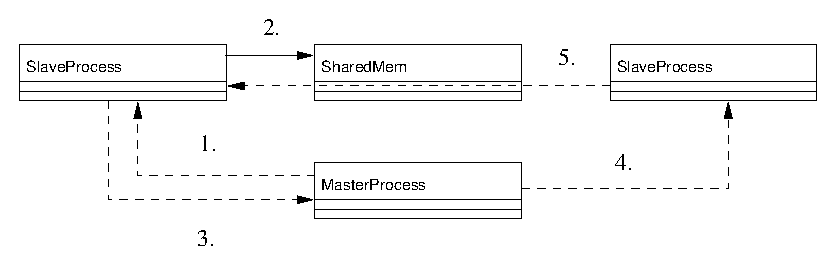
\includegraphics[width = \textwidth]{croute}
\caption{Kreiranje veze izme�u dvaju \texttt{SlaveProcess}-a na istom ra�unalu}
\label{sl:croute}
\end{center}
\end{figure}


\subsection{Dekkerov algoritam}
\label{subsec:dekker}

Za rje�avanje mogu�ih sukoba izme�u dvaju procesa koji se javljaju pri
istovremenom pristupu dijeljenoj memoriji kori�ten je
\textit{Dekkerov algoritam}.
Slijedi njegov kratak opis u kojem se zbog op�enitosti primjene algoritma
operacija �itanja ili upisivanja u dijeljenu memoriju naziva
\textit{kriti�nim odjeljkom}.\\


Za sinhronizaciju dvaju procesa Dekkerov algoritam koristi tri varijable.
Ove tri varijable prikazane su na
slici~\ref{sl:shm_lock_t}
u strukturi
\texttt{shm\_lock\_t}.

\begin{figure}
\begin{center}
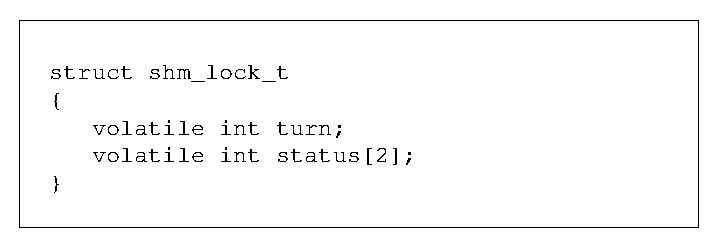
\includegraphics[width = 0.7\textwidth]{shm_lock_t}
\caption{Struktura \texttt{shm\_lock\_t}}
\label{sl:shm_lock_t}
\end{center}
\end{figure}

Varijabla
\texttt{turn}
mo�e poprimiti dvije vrijednosti - nulu ili jedinicu, ovisno o tome koji
od dvaju procesa ima pravo pristupa kriti�nom odjeljku prilikom sukoba. U
ovom primjeru, zbog bolje samodokumentacije
k\^oda,
umjesto nule i jedinice kori�tene su simboli�ke vrijednosti
\texttt{writer}
i
\texttt{reader}
(s obzirom da jedan od procesa isklju�ivo upisuje poruku u segment dijeljene
memorije, dok drugi iz istog segmenta isklju�ivo �ita poruke).
Varijabla
\texttt{status}
je
\textit{polje}
od dvije logi�ke vrijednosti koje se inicijalno postavljaju na nulu. Kada
bilo koji od dvaju procesa namjerava pristupiti kriti�nom odjeljku, svoju
varijablu
\texttt{status}
postavlja u jednicu. Iz istih razloga, opet nisu kori�tene broj�ane
vrijednosti ve� simboli�ke i to
\texttt{unlocked}
za nulu i
\texttt{locked}
za jedinicu.

Algoritam prikazan na
slici~\ref{sl:lock}
je jednostavan ako samo jedan proces pristupa kriti�nom odjeljku. U ovom
slu�aju on postavlja svoju
\texttt{status}
varijablu na vrijednost
\texttt{locked}
i provjerava vrijednost
\texttt{status}
varijable drugog procesa. Ako je ovaj
\texttt{unlocked},
tada nema nikakvih sukoba u pristupu i prvi proces nesmetano ulazi u kriti�an
odjeljak.
Ako drugi proces sada poku�a pristupiti kriti�nom odjeljku, otkrit �e da se
u njemu trenutno nalazi prvi proces i vrtit �e se u unutra�njoj ili vanjskoj
\texttt{while}
petlji, ovisno o vrijednosti varijable
\texttt{turn},
sve dok prvi proces ne napusti kriti�an odjeljak.

Kada oba procesa u�u u
\texttt{lock}
funkciju istovremeno da bi zatra�ili pristup kriti�nom odjeljku, oba �e
postaviti svoju
\texttt{status}
varijablu stanje
\texttt{locked}.
Tada �e primijetiti da drugi proces tako�er poku�ava ostvariti pristup
kriti�nom odjeljku i koristit �e varijablu
\texttt{turn}
da bi odredili koji ima pravo pristupa.
\textit{Gubitnik}
se povla�i i vrti se u
\texttt{while}
petlji sve dok drugi ne zavr�i. Klju�ni element ovog algoritma je da se iz
\texttt{lock}
funkcije ne izlazi sve dok vrijednost
\texttt{status}
varijable drugog procesa ne indicira da ovaj nema namjeru pristupiti kriti�nom
odjeljku.

Prilikom izlaska iz kriti�nog odjeljka proces poziva funkciju prikazanu na
slici~\ref{sl:unlock}.
I
\texttt{status}
i
\texttt{turn}
varijabla moraju se propisno postaviti tako da drugi proces bude u stanju da
iza�e iz obje
\texttt{while}
petlje u
\texttt{lock}
funkciji.

\begin{figure}
\begin{center}
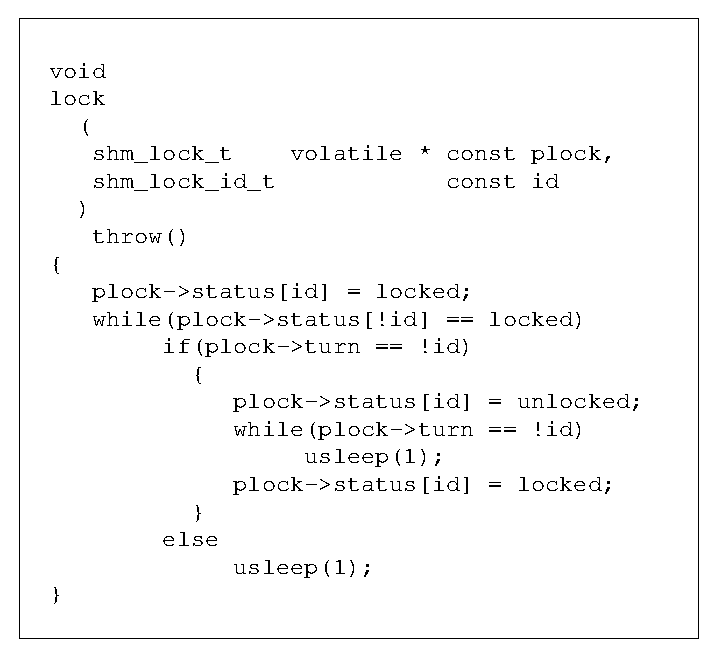
\includegraphics[width = 0.7\textwidth]{lock}
\caption{Zahtijevanje pristupa kriti�nom odjeljku}
\label{sl:lock}
\end{center}
\end{figure}


\begin{figure}
\begin{center}
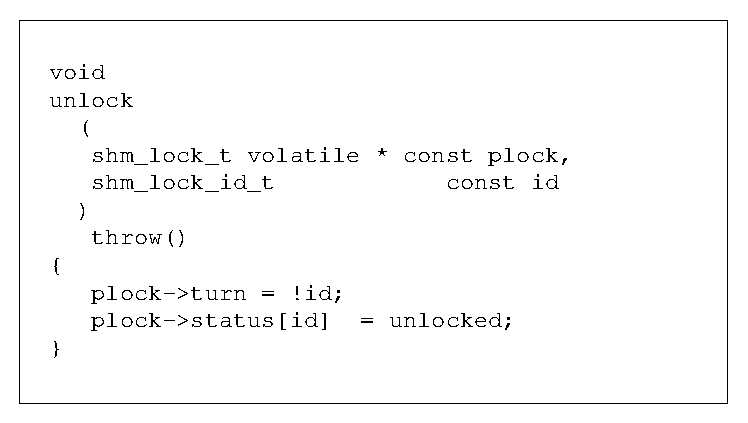
\includegraphics[width = 0.7\textwidth]{unlock}
\caption{Izlazak iz kriti�nog odjeljka}
\label{sl:unlock}
\end{center}
\end{figure}

\newpage


\section{Detalji implementacije komunikacije TCP/IP\\ protokolom}

Implementacija ovog dijela biblioteke nije zahtijevala toliko truda koliko
komunikacija dijeljenom memorijom s obzirom da se operacije �itanja i pisanja
na TCP/IP vezu
obavljaju pozivima standardnih funkcija
\texttt{read}
i
\texttt{write}
respektivno. Implementacija ovih dviju rutina je naravno skrivena pa se
njihov korisnik uglavnom nema o �emu brinuti osim njihovog pravovremenog
poziva.


\subsection{Razmjena poruka}

S obzirom na razli�itosti komunikacije TCP/IP-om i dijeljenom memorijom
zaglavlje poruke vi�e ne izgleda kako je prikazano na
slici~\ref{sl:message}
jer vi�e nisu potrebne varijable za sinhronizaciju, a nije potrebna ni
varijabla koja indicira da li je poruku pro�itana ili ne.
Dakle, zaglavlje poruka koje se prenose TCP/IP-om sadr�i isklju�ivo polja
\texttt{mid}
i
\texttt{len}.
Proces koji prima sada prvo pro�ita zaglavlje poruke na temelju kojeg odlu�i
koliko jo� mora pro�itati bajtova koji �ine njeno tijelo.


\subsection{Kreiranje novih procesa}

Ovaj se postupak odvija na na�in sli�an onom opisanom u
odjeljku~\ref{subsec:knp},
ali jednostavnije.
\texttt{MasterProcess}
prvo otkriva IP adresu stroja na kojem se nalazi. Nakon toga, od kernela
zatra�i da mu se dodijeli slobodan
\textit{port}.
Sada na dobivenoj adresi i port-u
\texttt{MasterProcess}
po�inje s
\textit{oslu�kivanjem},
tj.~po�inje se pona�ati kao
\textit{server}
�ekaju�i na zahtjeve
\textit{klijenata}
za spajanjem.
Dotle pokre�e
\texttt{SlaveProcess}
kojemu kao argumente komandne linije proslje�uje svoju IP adresu i port.
Pokrenuti
\texttt{SlaveProcess}
se sada spaja na server,
tj.~\texttt{MasterProcess},
koji naposljetku prihva�a klijentov zahtjev. Ovdje nije potrebno nikakvo
slanje inicijalnih poruka koje bi ozna�avale kraj uspje�nog ostvarivanja
veze jer je ova razmjena realizirana kroz
\textit{three-way handshake}
TCP protokola.


\subsection{Funkcije \texttt{read} i \texttt{write}}

Standardne funkcije
\texttt{read}
i
\texttt{write}
kori�tene s
\textit{deskriptorima veze}
onakvima kakvi jesu,
\textit{blokiraju}.
To zna�i da ako proces pozove funkciju
\texttt{read},
a nema novih podataka dostupnih za �itanje, funkcija
\textit{vra�a}
tek kada pristignu novi podaci. Jednako tako, ako se pozove funkcija
\texttt{write}
dok je spremnik procesa koji bi trebao primiti podatke prepunjen,
\texttt{write}
blokira sve dok primatelj ne pro�ita ono �to mu se nalazi u spremniku �ime
ga osloba�a za upis novih podataka. O�ito je da ovaj problem mo�e uvelike
naru�iti performanse aplikacije koja bi koristila biblioteku implementiranu na
ovakav na�in. Problem je rije�en na na�in da se funkcijom
\texttt{fcntl}
deskriptori veze postave za
\textit{neblokiraju�e}.
Sada pozivi funkcija
\texttt{read}
i
\texttt{write}
vra�aju odmah u slu�aju da ne mogu biti udovoljeni postavljaju�i globalnu
varijablu
\texttt{errno}
u odgovaraju�e stanje
(\texttt{EWOULDBLOCK},
odnosno u nekim implementacijama
\texttt{EAGAIN}).
Stoga su ove dvije funkcije
\textit{omotane}
u rutinama koje se snose s ovim detaljem
(slike~\ref{sl:readn}
i~\ref{sl:writen}).


\begin{figure}
\begin{center}
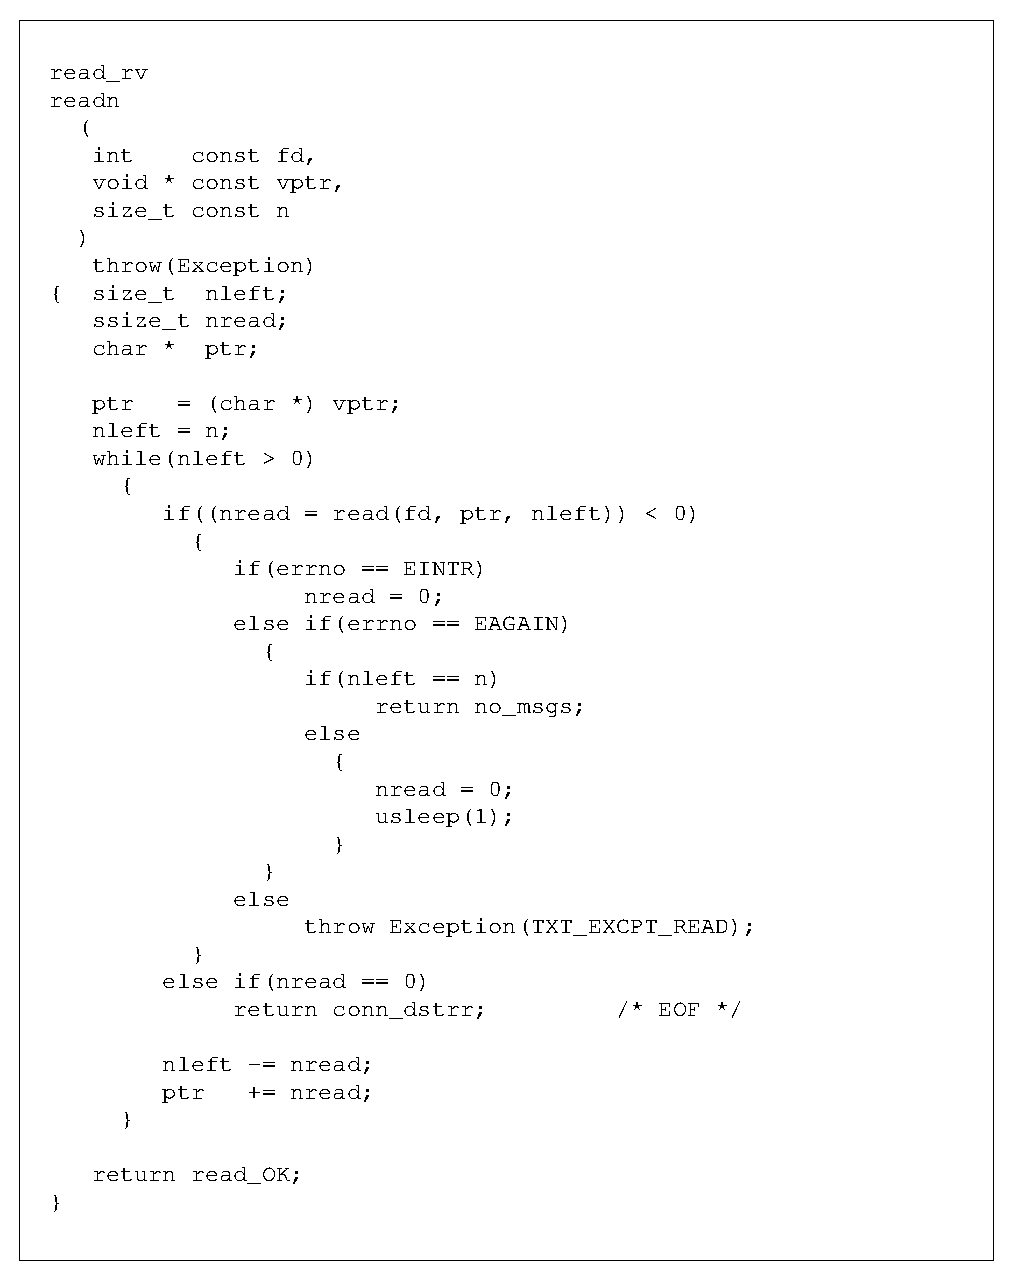
\includegraphics[width = \textwidth]{readn}
\caption{\textit{Wrapper} \texttt{read} funkcija}
\label{sl:readn}
\end{center}
\end{figure}

\begin{figure}
\begin{center}
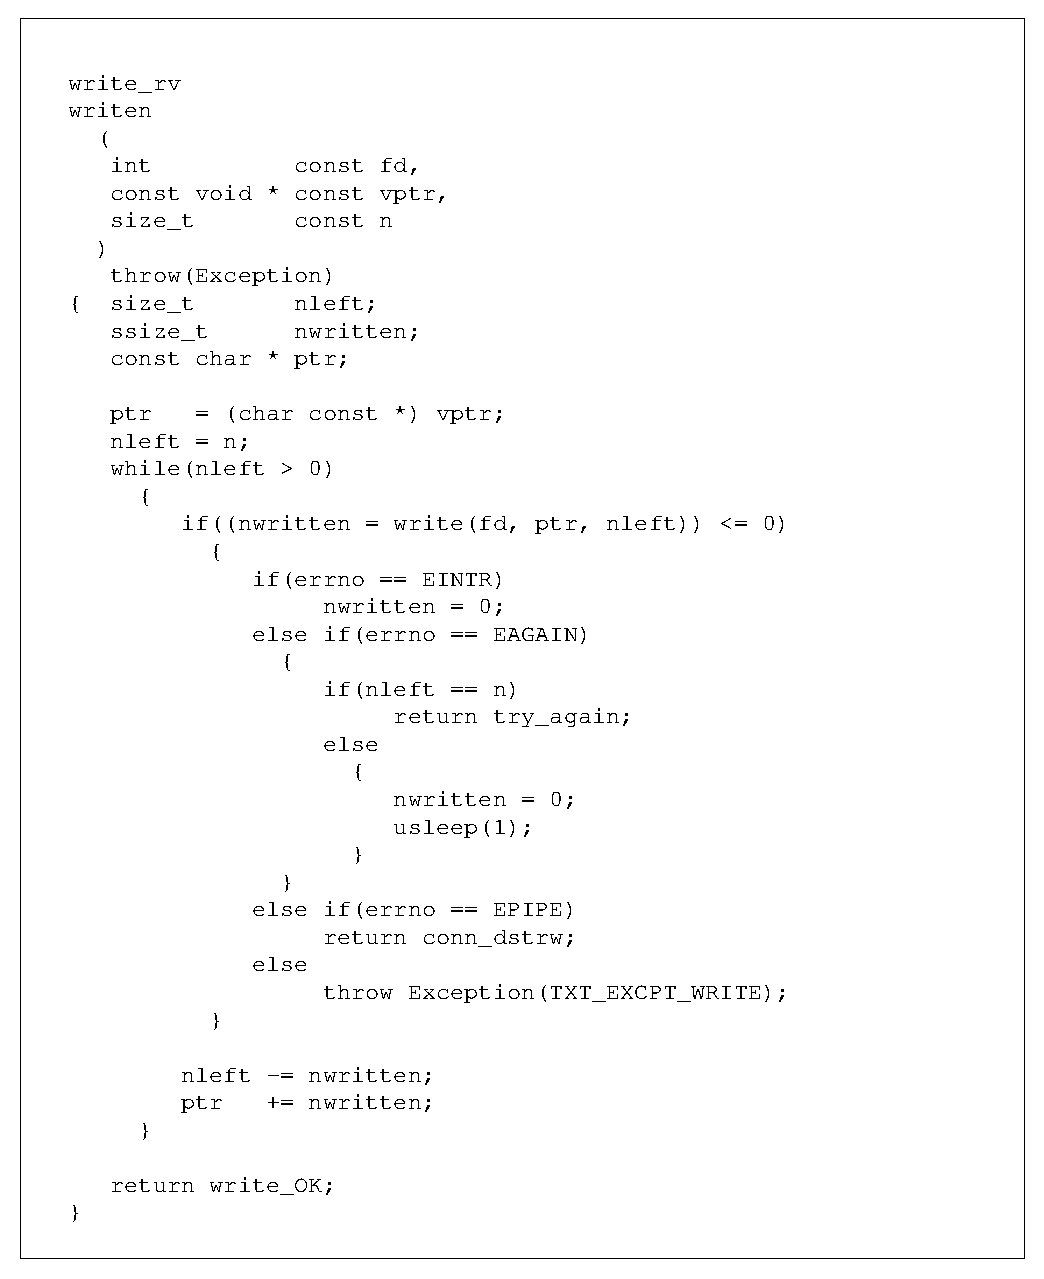
\includegraphics[width = \textwidth]{writen}
\caption{\textit{Wrapper} \texttt{write} funkcija}
\label{sl:writen}
\end{center}
\end{figure}


Za primijetiti je da ove dvije
\textit{wrapper}
funkcije vode ra�una o jo� nekim detaljima. Jedan od njih je slu�aj u kojem
primljeni
\textit{signal}
prekida poziv
\texttt{read}
ili
\texttt{write}
funkcije. Ovaj slu�aj se detektira zahvaljuju�i tome �to je
\texttt{errno}
postavljen na
\texttt{EINTR}.
Kada se ova situacija pojavi, potrebno je nanovo pozvati odabranu funkciju.
Tako�er je mogu�e i to da
\texttt{read}
ili
\texttt{write}
funkcija ne obave svoj posao u cijelosti. Npr.~od funkcije
\texttt{read}
mo�emo zatra�iti da pro�ita deset bajtova, a ova ih pro�ita pet iz razloga
�to ostalih pet jo� nije pristiglo do onog trenutka kada je funkcija pozvana.
Ili ako npr.~od funkcije
\texttt{write}
zatra�imo da upi�e deset bajtova, a ova ih upi�e samo pet iz razloga �to
ostalih pet nije moglo stati u me�uspremnik. Bitno je naglasiti da su ova
dva slu�aja razli�ita od onih u kojima se opisuje blokiranje
\texttt{read}
i
\texttt{write}
funkcija iz razloga �to se ovdje ipak vr�i neko (mada ne cjelovito) �itanje,
tj.~upisivanje.

\chapter{Testiranje}

\section{Uvod}

Kori�tenjem razvijene biblioteke napisan je niz programa namijenjen upravo
njenom testiranju. Ovih ne�to vi�e od sedam stotina linija
k\^oda
dijelom slu�i pronala�enju pogre�aka u biblioteci, a dijelom samom
mjerenju njenih performansi. Kroz ostatak ovog poglavlja bit �e rije�i
isklju�ivo o posljednjim aplikacijama i rezultatima koji su njima dobiveni.

\section{Mjerenje performansi biblioteke}

Mjerenja su obavljena na ra�unalima
\texttt{lolek.fesb.hr}
i
\texttt{bolek.fesb.hr}
od kojih je svako opremljeno sa po dva
\textit{Intel PIII}
procesora na 600 MHz, dok su me�usobno povezana 100Mb/s
\textit{ethernet}-om. Testiranja su se nastojala obaviti na �to
manje optere�enim strojevima, dakle kada je aktivnost drugih korisnika na
njima bila minimalna.\\

Za prora�une vremena ka�njenja i propusnosti veze (u funkciji veli�ine poruke)
kori�teni su programi
\texttt{bechmark}
i
\texttt{tcp\_benchmark},
za komunikaciju dijeljenom memorijom odnosno TCP/IP-om respektivno.

Programi
\texttt{matrix}
i
\texttt{pmatrix}
su napisani za ilustraciju opravdanosti emulacije paralelnog ra�unala.

Sva �etiri programa prilo�ena su zajedno s
k\^odom.


\subsection{Vrijeme ka�njenja poruke}

Mjerenja su obavljena na na�in da je jedan proces, nakon �to bi poslao
poruku, �ekao da mu je drugi proces vrati. Da bi se dobili �to to�niji
rezultati, ovaj postupak se ponavljao za svaku poruku po tisu�u puta.
Mjerilo se ukupno utro�eno vrijeme koje je tada dijeljenjem dalo vrijeme
ka�njenja poruke
(slike~\ref{sl:shmem_bnch} i~\ref{sl:tcp_bnch}).
Propusnost
(slike~\ref{sl:shmem_bndw} i~\ref{sl:tcp_bndw})
je dobivena tako da se ovim vremenom podijelila veli�ina poruke. S obzirom da
je tijelo korisni�ke poruke kod komunikacije dijeljenom memorijom ograni�eno,
mjerenja su obavljena samo za veli�ine poruka od 0 do 2024 bajta.

\subsubsection{Dijeljena memorija}
\label{subsubsec:dm}

Rezultate dobivene za dijeljenu memoriju ne treba posebno komentirati. Oni
prvenstveno ovise brzinama izvo�enja standardnih funkcija za kopiranje
blokova memorije. Jasno je da �e kopiranje biti br�e �to je blok, odnosno
korisni�ka poruka manja. Ostatak utro�enog vremena otpada na sinhronizaciju
procesa i izmjenu konteksta. Bitno je samo jo� jednom naglasiti da se ovdje
radi o situaciji u kojoj proces odmah nakon slanja poruke �eka na odgovor. Kada
bi bilo rije�i o uzastopnom slanju ve�ih poruka, s obzirom na ograni�enu
veli�inu dijeljenog spremnika, ovaj vid komunikacije bi mogao predstavljati i
\textit{usko grlo}
i to iz razloga u�estalijih sukoba procesa nastalih zbog istovremenog pristupa
zajedni�kom segmentu, odnosno zbog njihove ote�ane sinhronizacije.\\


\subsubsection{TCP/IP protokol}

Slika~\ref{sl:tcp_bnch}
zahtijeva poja�njenje. Vidljivo je da male (od 0 do otprilike 600 bajtova) i
velike (preko otprilike 1500 bajtova) poruke imaju veliko ka�njenje, dok je
ka�njenje poruka srednje veli�ine znatno manje.

Ka�njenje malih poruka uvjetovano je
\textit{delayed ACK}
i
\textit{Nagleovim algoritmom}
te njihovom interakcijom, dok je ka�njenje velikih poruka uvjetovano njihovom
\textit{fragmentacijom}.\\

\textit{Delayed ACK}
algoritam djeluje tako da sprje�ava TCP u slanju potvrda primitka �im podaci
pristignu na svoje odredi�te. Umjesto toga, TCP sada �eka neko kratko vrijeme
pa tek onda �alje potvrdu. Naime, za o�ekivati je da �e se u ovom vremenskom
intervalu pojaviti podaci koje treba poslati nazad na drugi kraj veze. Tada bi
se potvrda primitka poslala zajedno s tim podacima i na taj bi se na�in
izbjegao prijenos jednog dodatnog TCP segmenta.

Svrha Nagleovog algoritma je da se, zbog pove�anja iskoristivosti, smanji broj
malih paketa na mre�i. Ovaj algoritam nala�e da se nekom vezom ne �alju mali
paketi sve dok ne pristignu potvrde primitka za sve do tada poslane podatke.

Dakle, u na�em slu�aju situacija je sljede�a. TCP/IP vezom server klijentu
prvo �alje zaglavlje poruke na temelju kojeg klijent odre�uje koliko jo�
bajtova sa�injava tijelo poruke. Po�to klijent serveru u me�uvremenu ne �alje
nikakve podatke, zbog
\textit{delayed ACK}
algoritma neko vrijeme izostaje potvrda primitka zaglavlja poruke. Dok traje
ovaj vremenski interval, server zbog Nagleovog algoritma ne �alje tijelo
poruke jer ovo predstavlja mali paket. Da je rije� o velikom paketu, ovaj bi
se normalno poslao klijentu bez �ekanja potvrde primitka zaglavlja poruke, kao
�to je slu�aj s porukama srednje veli�ine. Kada napokon istekne vremenski
interval
\textit{delayed ACK}
algoritma, klijent �alje potvrdu primitka zaglavlja poruke pa server tek tada
�alje njeno tijelo.\\

Maksimalna veli�ina paketa koja se prenosi
\textit{ethernet}-om
iznosi 1500 bajtova. S obzirom da veli�ina TCP i IPv4 zaglavlja zajedno
minimalno iznosi 40 bajtova, TCP segmenti su obi�no veliki do 1460
bajtova. Ako se �alje poruka ve�a od TCP segmenta, tada se ona
\textit{fragmentira}
na blokove spomenute veli�ine te se dalje mre�om prenosi dio po dio, pa je
stoga potrebno i vi�e vremena za njen prijenos.
Slika~\ref{sl:tcp_bnch}
zorno ilustrira ovu situaciju. Skok u ka�njenju jasno je vidljiv kod veli�ine
poruke koja odgovara TCP segmentu. Konkretno, prijenos poruka koje nisu
zahtijevale fragmentaciju bio je trostruko br�i od ovih fragmentiranih.


\begin{figure}[p]
\begin{center}
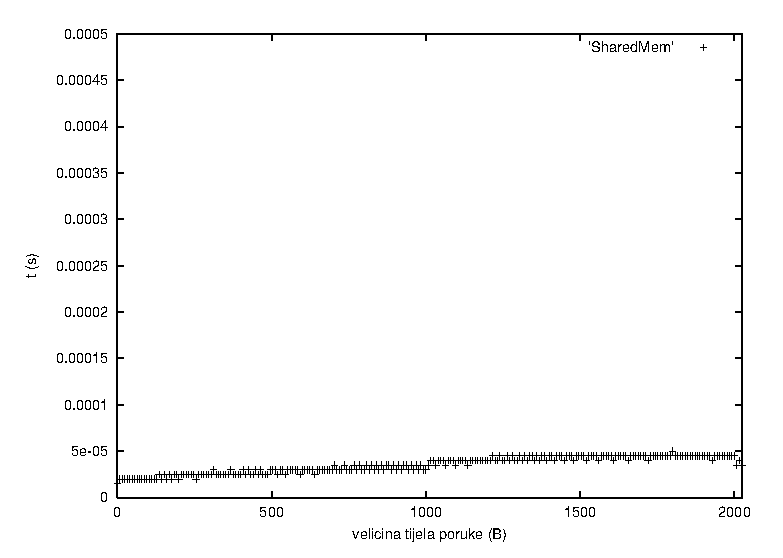
\includegraphics{shmem_bnch}
\end{center}
\caption{Ka�njenje poruke kod komunikacije dijeljenom memorijom}
\label{sl:shmem_bnch}
\end{figure}


\begin{figure}[p]
\begin{center}
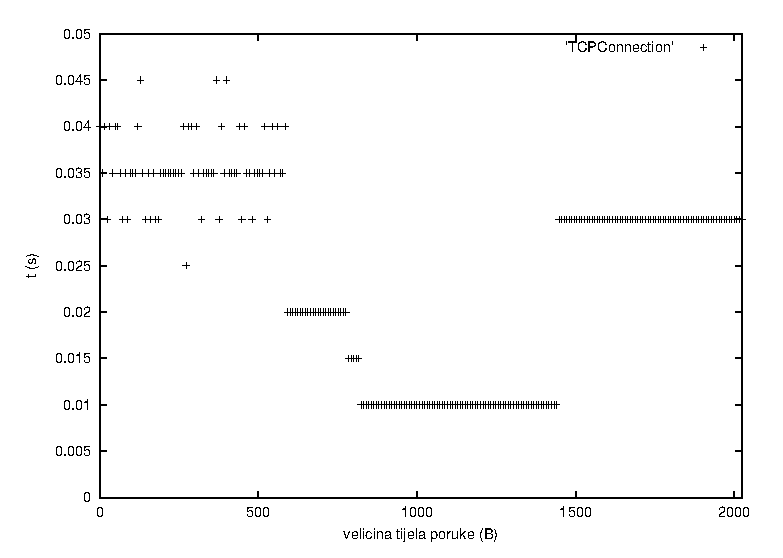
\includegraphics{tcp_bnch}
\end{center}
\caption{Ka�njenje poruke kod komunikacije TCP/IP-om}
\label{sl:tcp_bnch}
\end{figure}


\begin{figure}
\begin{center}
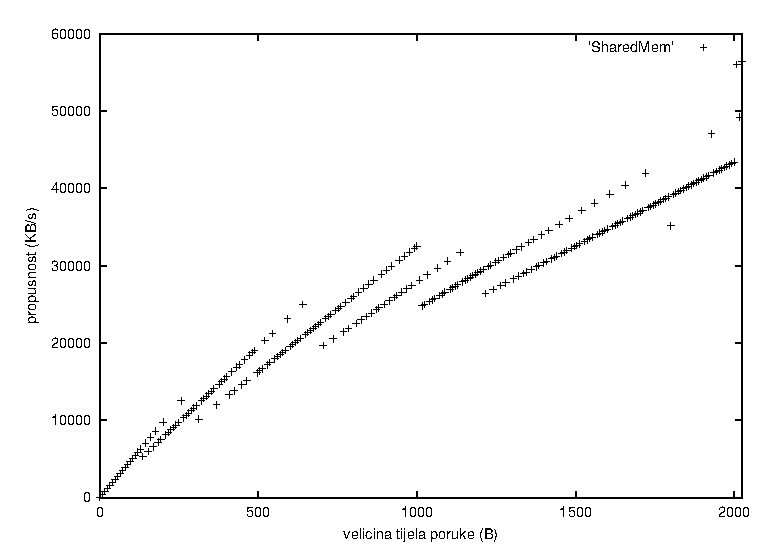
\includegraphics[]{shmem_bndw}
\end{center}
\caption{Propusnost dijeljene memorije}
\label{sl:shmem_bndw}
\end{figure}


\begin{figure}
\begin{center}
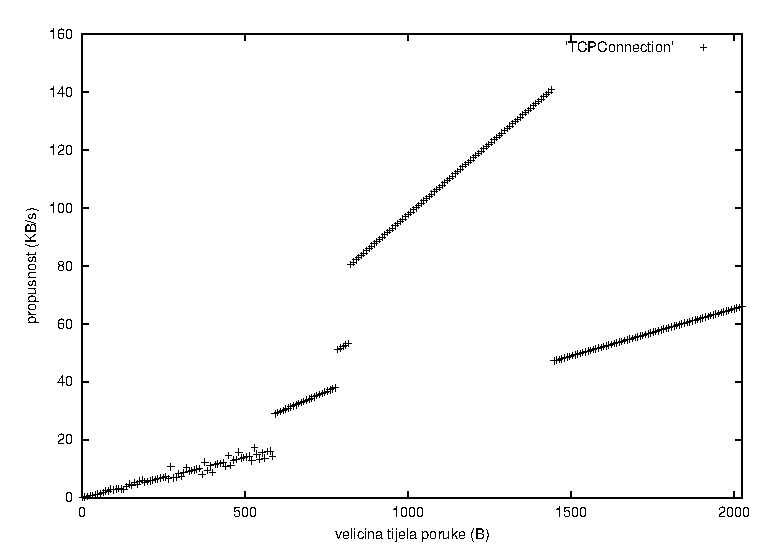
\includegraphics[]{tcp_bndw}
\end{center}
\caption{Propusnost TCP/IP-a}
\label{sl:tcp_bndw}
\end{figure}

\newpage
\subsection{Primjer: mno�enje matrica}

Za ilustraciju opravdanosti emulacije paralelnog ra�unala, kori�tenjem
razvijene biblioteke, realizirana je aplikacija namijenjena mno�enju matrica.
Matrice su sa�injavali brojevi (s pomi�nim zarezom) jednostruke preciznosti.
Da bi se pove�ao broj operacija nad ovim tipom podatka i na taj se na�in
istaklo vrijeme prora�una nad vremenom prijenosa matrice, tra�io se rezultat
izraza
$ \log A^{m \times n} \times \log B^{n \times m}$.
Dobivena vremena prora�una za zadane dimenzije matrica i broj procesa
uklju�enih u obradu prikazana su u
tablici~\ref{tbl:matrice}.
Za slu�ajeve kada se emuliralo paralelno ra�unalo, mno�enje matrica se
obavljalo na na�in da je
\textit{master}
proces svim pokrenutim
\textit{slave}-ovima
prvo prenio �itavu drugu (B) matricu i to stupac po stupac, zatim im podijelio
retke prve (A) matrice i naposljetku �ekao rezultate prora�una, odnosno retke
kona�ne matrice.

\subsubsection{\textit{local}}

Prvi (referentni) stupac sadr�i vremena potrebna za obavljanje zadatka
lokalno, na jednom procesoru. Za primijetiti je da ovaj primjer daje
optimalno vrijeme prora�una za mali broj operacija.

\subsubsection{\textit{2 $ \times $ ShMem}}

U drugom stupcu navedeni su rezultati prora�una izvedenog tako�er na jednom
ra�unalu, ali su sada mno�enje obavljala dva procesa vezana dijeljenom
memorijom. Dakle, u ovom slu�aju obrada je uposlila oba raspolo�iva procesora.
Iz tablice je vidljivo da su za mali broj podataka (tj.~operacija s pomi�nim
zarezom) postignuti lo�i rezultati iz razloga �to je prijenos podataka oduzeo
vi�e vremena od samog prora�una. Za ve�e dimenzije matrica to nije bio slu�aj,
pa su se ovdje mno�enja obavljala u vremenskim intervalima kra�ima i do
49\%
od ekvivalentnog referentnog primjera.

\subsubsection{\textit{2 $ \times $ TCP}}

U sljede�em stupcu navedeni su rezultati prora�una u kojem su se koristili
resursi oba ra�unala. Na jednom se nalazio
\textit{master}
proces, koji bi pokrenuo druga dva
\textit{slave}
procesa na udaljenom ra�unalu te s njima ostvario vezu TCP/IP-om. Iz
rezultata je vidljivo da je za mali broj podataka ova kombinacija najsporija
�to nije iznena�enje s obzirom da je potrebno najvi�e vremena za ostvarivanje
veza, inicijalizaciju procesa i sami prijenos malih paketa. Kod veli�ine
preno�enih stupaca matrice za koju TCP/IP ima najve�u propusnost
(slika~\ref{sl:tcp_bndw})
postignuti su rezultati bolji od prethodnog slu�aja u kojem se komunikacija
obavljala dijeljenom memorijom. Osim najve�e propusnosti TCP/IP-a, ovo vrijeme
(duplo kra�e od referentnog) je postignuto i zbog toga �to je
\textit{master}
proces izoliran na jednom ra�unalu i svojim izvo�enjem ne usporava sami
prora�un koji se u potpunosti obavlja na drugom ra�unalu. Rezultati dobiveni
za ve�e dimenzije matrica usporedivi su s onima iz prethodnog stupca iz
razloga obja�njenog u
odjeljku~\ref{subsubsec:dm}.

\subsubsection{\textit{2 $ \times $ TCP, 2 $ \times $ ShMem}}

Ova kombinacija procesa dala je o�ekivane rezultate za sve dimenzije
matrica. Za male matrice vremena izvo�enja su bila izme�u onih prikazanih u
prethodna dva stupca. S obzirom da su sada u mno�enju sudjelovala sva �etiri
raspolo�iva procesora, vrijeme prora�una u najboljem slu�aju je skra�eno na
svega
26\%
onog referentnog.



\begin{table}
\begin{center}
\begin{tabular}{|c||c|c|c|c|}
\hline
$ m \times n $     & local  & 2 $ \times $ ShMem & 2 $ \times$ TCP  & 2 $\times$ TCP, 2 $ \times$ ShMem \\
\hline
\hline
$ 3 \times 4   $   & 0      & 0.01               & 0.21 	    & 0.19   \\
\hline
$ 30 \times 40 $   & 0.04   & 0.03  		 & 0.23 	    & 0.21   \\
\hline
$ 30 \times 80 $   & 0.08   & 0.06  		 & 0.24 	    & 0.21   \\
\hline
$ 60 \times 80 $   & 0.32   & 0.21  		 & 0.36	 	    & 0.38   \\
\hline
$ 60 \times 120 $  & 0.49   & 0.29  		 & 0.44 	    & 0.33   \\
\hline
$ 90 \times 120 $  & 1.09   & 0.62  		 & 0.88 	    & 0.52   \\
\hline
$ 90 \times 240 $  & 2.18   & 1.17  		 & 1.41 	    & 0.89   \\
\hline
$ 180 \times 240 $ & 8.76   & 4.53  		 & 4.64 	    & 2.57   \\
\hline
$ 180 \times 340 $ & 12.42  & 6.37      	 & 6.52 	    & 3.61   \\
\hline
$ 280 \times 340 $ & 30.09  & 21    		 & 15.01 	    & 11.81  \\
\hline
$ 280 \times 440 $ & 38.82  & 27.07  		 & 19.34 	    & 15.85  \\
\hline
$ 380 \times 440 $ & 71.61  & 36.18  		 & 36.65 	    & 18.65  \\
\hline
$ 380 \times 500 $ & 81.26  & 41.42  		 & 41.75 	    & 22.65  \\
\hline
$ 500 \times 500 $ & 140.58 & 71.49 		 & 71.89 	    & 37.06  \\
\hline
\end{tabular}
\end{center}
\caption{Vrijeme (u s.)~potrebno za mno�enje
$\log A^{m \times n} \times \log B^{n \times m}$}
\label{tbl:matrice}
\end{table}

\chapter{Zaklju�ak}

Zahvaljuju�i aplikacijama �ije izvo�enje zahtijeva sve vi�e procesorskog
vremena, emulacija paralelnog ra�unala ima svoje opravdanje. Konkretni
rezultati dobiveni kori�tenjem realizirane biblioteke
(tablica~\ref{tbl:matrice}
na
strani~\pageref{tbl:matrice})
potvr�uju isplativost upotrebe takvog sustava. Naravno, o�ito je da njegove
prednosti dolaze do izra�aja isklju�ivo u situacijama kada je primjena
opravdana, odnosno kada je samo vrijeme obrade podataka ve�e od vremena
potrebnog da se ti isti podaci distribuiraju me�u procesima.


\section{Smjernice budu�eg razvoja biblioteke}

Sa svojih preko �etiri tisu�e linija
k\^oda
biblioteka je cjelovita u tolikoj mjeri koliko joj je to dozvolio nazna�eni
rok. Sadr�i osnovnu funkcionalnost potrebnu za emulaciju paralelnog
ra�unala te bi, s obzirom na postignute rezultate prikazane u prethodnom
poglavlju, mogla prona�i i jednostavniju prakti�nu upotrebu. No, od ozbiljnih
proizvoda na tom podru�ju je dijeli dosta toga. Kroz ostatak ovog odjeljka
izneseno je nekoliko osnovnih ideja kojima bi bilo posve�eno daleko vi�e
pa�nje da je bilo vi�e vremena. No s obzirom na dragocjenost ovog iskustva
nije isklju�ena ni mogu�nost da u skorom vremenu te ideje budu i
implementirane
\ldots

\subsection{Dizajn}

Trenutni dizajn biblioteke je sasvim zadovoljavaju�, no neke preinake bi
itekako pridonijele boljoj organizaciji
k\^oda
i u�inile ga prikladnijim za upotrebu i u drugim projektima. Konkretno,
u klasi
\texttt{Process}
i svim deriviranima iz nje, implementirane su aktivnosti koje iziskuju
komunikacija i dijeljenom memorijom i TCP/IP-om. Idealno bi bilo kada bi se
ove funkcionalnosti razdvojile u posebne module.

Tako�er, kod klase
\texttt{Process}
se zbila stanovita dizajnerska pogre�ka zbog koje je skrivanje njene
implementacije
(odjeljak~\ref{subsec:si})
nepotpuno. Da bi se izbjegli
\texttt{protected}
atributi prijeko je potreban redizajn.


\subsection{Implementacija dodatnih metoda}

Premda je, po mom mi�ljenju, postignuta jednostavnost su�elja, mo�e se re�i da
metode trenutno implementiranih klasa pru�aju prije asketsko nego komotno 
okru�enje. Za svaku od implementiranih klasa, a poglavito za API, postoji jo�
hrpa metoda koje bi, da su implementirane, dodatno pojednostavnile
kori�tenje biblioteke. Jasno, njihov popis je predug da bi se ovdje navodio.

\subsection{Komunikacija dijeljenom memorijom}

Prema rezultatima iz prethodnog poglavlja, za odre�ene primjene segment
dijeljene memorije se pokazao nedovoljno velikim. Najbolje rje�enje bi bilo da
korisnik sam odabire veli�inu ovog komunikacijskog kanala ovisno o vlastitoj
procjeni. Tako�er, trenutni veliki nedostatak je i to �to, za razliku od
komunikacije TCP/IP-om, postoji kona�no dozvoljena veli�ina poruke.
Biblioteka bi djelovala ozbiljnije kada bi se poruke �ija veli�ina nadma�uje
veli�inu segmenta dijeljene memorije slale dio po dio te se na prijemnoj
strani nazad sastavljale.

\subsection{Dojava pogre�ki}

Premda je to u UNIX
f\mbox{}ilozof\mbox{}iji
posve uobi�ajena praksa, smatram da bi bilo
bolje kada se poruke o korisni�kim pogre�kama po�injenim tijekom rada
biblioteke ne bi ispisivale direktno na konzolu
\texttt{cerr}.
Ispis na konzolu bi mo�da mogla biti jedna od mogu�ih opcija, dok bi za neku
graf\mbox{}i�ku
aplikaciju bilo podesnije ispisivanje poruka npr.~na to�no odre�enim
koordinatama zaslona. Ovoj mogu�nosti bi se moglo izi�i u susret uvo�enjem
posebne klase koja bi pamtila tekstualne poruke o pogre�kama, koje bi tada
korisnik mogao prikazati na na�in kako on to �eli.

\subsection{Signali}

Da bi se izbjegli problemi koji mogu nastati zbog razlika me�u
implementacija UNIX operacijskih sustava, za
\textit{bu�enje}
procesa je kori�ten signal
\texttt{SIGUSR2}.
Podesnije rje�enje bi predstavljalo kori�tenje
\texttt{SIGIO}
signala �ime bi se
\texttt{SIGUSR2}
vratio na raspolaganje korisniku biblioteke. U nekoj budu�oj verziji bi se
trebalo vi�e pozabaviti i s ovim pitanjem.\newpage


\section{Posljednja rije�}

Izrada ovog rada bila je dragocjeno iskustvo iz vi�e razloga. Kroz taj proces
su se sa�ela i konkretizirala ve�ina predavanja s posljednje godine studija.

Zahvaljuju�i samoj temi po prvi put sam se susreo s pojmovima i problemima
vezanim uz paralelnu obradu podataka, pri �emu su mi posebno zadovoljstvo
pru�ala vlastita idejna rje�enja.

Zanimljivosti je tako�er pridonio i objektno orijentirani pristup �itavom
problemu zbog kojega je moje dotada�nje znanje vezano uz tu popularnu
metodologiju u�inilo znatan korak naprijed. Ni�ta manje nisu vrijedna ni
iskustva s programskim jezikom C++. Jednako tako, kroz ovaj rad je realiziran
moj do sada najve�i programerski projekt pa je na konkretnom primjeru mnogo
toga nau�eno i o odr�avanju
k\^oda
\textit{pod kontrolom}.

Tijekom rada sam se pobli�e upoznao i sa
specif\mbox{}i�nostima
UNIX operacijskog
sustava, kako promatranog s aspekta korisnika tako i s aspekta programera.
Posljednje se poglavito odnosi na pojmove dijeljene memorije i signala.

Kraj, tj.~formatiranje samog dokumenta zabavnijim je u�inio
\LaTeX{}.\\

Posljednju re�enicu u diplomskom radu �u iskoristiti da se zahvalim GNU
projektu i ljudima koji stoje iza njega.

\begin{thebibliography}{99}
\addcontentsline{toc}{chapter}{Bibliograf\mbox{}ija}

\bibitem{MA} Curt Schimmel:
\textit{UNIX Systems for Modern Arhitectures -\\
Symetric Multiprocessing and Caching for Kernel Programmers}\\
Addison-Wesley; 1994.

\bibitem{APUI} W.~Richard Stevens:
\textit{Advanced Programming in the UNIX Environment}\\
Addison-Wesley; 1992.

\bibitem{UNP} W.~Richard Stevens:
\textit{UNIX NETWORK PROGRAMMING -\\
Networking APIs: Sockets and XTI (Vol.~1)}\\
Prentice-Hall; 1998.

\bibitem{CC} Steve McConnel:
\textit{Code complete}\\
Microsoft Press; 1994.

\bibitem{BE} Bruce Eckel:
\textit{Thinking in C++} (Vol.~1 \& 2, 
2nd
edition)\\
Prentice Hall; 2000.

\bibitem{IZ1} Ivan Zoraja:
\textit{Online Monitoring in Software DSM Systems}\\
(Research Report Series; Vol.~20)\\
LLR-Techniche 
Universit\"{a}t
M\"{u}nchen;
2000.

\bibitem{IZ2} I.~Zoraja, V.~Seitz, A.~Bode, P.~Slapni�ar:\\
\textit{Resource Management in Message Passing Environments}\\
(Journal of computing and information technology; Vol.~9, No.~1)\\
University Computing Centre Zagreb; 2001.

\bibitem{SGI}
\textit{Standard Template Library Programmer's Guide}\\
Silicon Graphics Computer Systems; 1996.

\bibitem{MAKE} Richard M.~Stallman 
\& 
Roland McGrath:
\textit{GNU Make}\\
Free Software Foundation; 1999.

\bibitem{EL} Jon Warbrick 
\& 
D.~Carlisle, M.~Goossens, S.~Rahtz, A.~Clark:\\
\textit{Essential 
\LaTeX{}
++}\\
1994.

\bibitem{NSHORT} T. Oetiker, H.~Partl, I.~Hyna 
\& 
E. Schlegl:\\
\textit{The Not So Short Introduction to \LaTeX2e{}}
(Ver.~3.7)\\
Free Software Foundation; 1999.

\end{thebibliography}


\end{document}
